% IJAMT draft based on the Springer Nature journal article template.
% Target journal: The International Journal of Advanced Manufacturing Technology.
\documentclass[pdflatex,iicol,sn-mathphys-num]{sn-jnl}

\usepackage{graphicx}
\usepackage{multirow}
\usepackage{amsmath,amssymb,amsfonts}
\usepackage{amsthm}
\usepackage{mathrsfs}
\usepackage[title]{appendix}
\usepackage{xcolor}
\usepackage{textcomp}
\usepackage{manyfoot}
\usepackage{booktabs}
\usepackage{algorithm}
\usepackage{algorithmicx}
\usepackage{algpseudocode}
\usepackage{array}
\usepackage{tabularx}
\usepackage{makecell}
\usepackage{stfloats}
\hypersetup{hypertexnames=false}

\raggedbottom

\begin{document}

\title[Graph-guided dual-population evolution for FJSP]{
  Graph-Guided Heterogeneous Dual-Population Evolution for Multi-Objective Flexible Job Shop Scheduling
}

\author[1]{\fnm{Changqi} \sur{Han}}\email{email-to-be-added}
\author*[1]{\fnm{Jie} \sur{He}}\email{email-to-be-added}
\author[1]{\fnm{Shihong} \sur{Duan}}\email{email-to-be-added}

\affil*[1]{\orgdiv{School of Computer and Communication Engineering}, \orgname{University of Science and Technology Beijing}, \orgaddress{\city{Beijing}, \postcode{100083}, \country{China}}}

% % 柔性作业车间调度（FJSP）是先进制造中的一类基础决策问题，每道工序都需同时进行工序排序并分配至其可选机器之一。
% % 实际生产须联合优化若干相互冲突的目标，即最大完工时间影响产出与交付、最大机器负荷反映瓶颈负载、总机器负荷关乎资源与能耗效率；因而制造方需要的是一组权衡方案而非单一解。
% % 多目标进化算法，尤其是非支配排序遗传算法 II（NSGA-II），适于该任务，因为单次运行即可返回一整组非支配调度方案；然而其性能仍受两点制约：初始种群通常随机或由固定派工规则生成，不含所求实例的先验知识；且单一种群需同时兼顾收敛性与多样性。
% % 基于"FJSP 实例的结构本身即揭示了哪些派工规则更可能有效"这一观察，本文离线学习该映射并用以初始化搜索：将每个实例表示为静态异构析取图，由结合边条件消息传递与全局注意力池化的图神经网络预测调度规则组合上的分布，得到面向实例的规则先验。
% % 该先验初始化两个互补的异构种群，一个促进广泛的 Pareto 前沿覆盖、另一个强化局部开发，并由双向交换机制与自适应混合进化策略进一步协调。
% % 在模拟实例与公共基准上的实验表明，所提框架在 hypervolume、IGD 及解分布指标上稳定优于单种群 NSGA-II 与同质双种群变体。
% \abstract{
%   Flexible job shop scheduling (FJSP) is a fundamental decision problem in advanced manufacturing, in which every operation must be simultaneously sequenced and allocated to one of its eligible machines. Practical production must jointly optimize several conflicting objectives, namely the makespan governing throughput and delivery, the maximum machine workload reflecting bottleneck load, and the total machine workload relating to resource and energy efficiency; consequently, a manufacturer needs a set of trade-off schedules rather than a single solution.
%   Multi-objective evolutionary algorithms, particularly the non-dominated sorting genetic algorithm II (NSGA-II), are well suited to this task, since a single run returns an entire set of non-dominated schedules. Their performance, however, remains constrained by two issues: the initial population is commonly produced at random or by fixed dispatching rules and therefore embeds no knowledge of the instance to be solved, while a single population is required to reconcile convergence and diversity at the same time.
%   Motivated by the observation that the structure of an FJSP instance already reveals which dispatching rules are likely to be effective, this study learns such a mapping offline and exploits it to initialize the search. Each instance is represented as a static heterogeneous disjunctive graph, and a graph neural network that combines edge-conditioned message passing with global attention pooling predicts a distribution over dispatching-rule combinations, yielding instance-specific rule priors.
%   These priors initialize two complementary heterogeneous populations, one promoting broad Pareto-front coverage and the other intensifying local exploitation, which are further coordinated through a bidirectional exchange mechanism and an adaptive mixed evolution strategy.
%   Experiments on simulated instances and public benchmarks demonstrate that the proposed framework consistently improves the hypervolume, IGD, and solution-distribution indicators over single-population NSGA-II and homogeneous dual-population variants.
% }

% 多目标冲突下的柔性作业车间调度（FJSP）是柔性制造中的一类核心决策问题；多目标进化算法对其颇具吸引力，因为单次运行即可返回一组权衡调度方案。
% 然而其有效性受两方面制约：随机或规则初始化的种群忽略实例特有结构，传统单种群结构又将收敛性与多样性耦合，使初始种群质量难以控制，最终帕累托前沿在质量与稳定性上均较弱。
% 为在上述两方面同时增强搜索，本文提出一种由实例特定学习先验引导的异构双种群进化优化方法：在离线阶段，结合全局注意力池化的边条件图神经网络将每个实例编码为静态异构析取图，并从多目标软标签中预测调度规则组合上的分布。
% 在在线阶段，该分布驱动两个互补种群的异构初始化：主种群依据完整的预测概率分布在多种规则组合上按比例分配个体以求广覆盖，探索种群只以概率最高的单一规则组合为种子做深度搜索；二者由双向交换与自适应混合进化协调。
% 在合成实例与公开的 BehnkeGeiger 基准上，仅所学先验即可使超体积相较随机初始化的 NSGA-II 提升 123.6\%，完整框架在此基础上再提升 30.8\%，并在两个数据集上于超体积、IGD 与分布稳定性（$\Delta$、$\Delta_v$）上均取得最优。
\abstract{
  Flexible job shop scheduling (FJSP) under multiple conflicting objectives is a core decision problem in flexible manufacturing, for which multi-objective evolutionary algorithms are attractive because a single run returns a set of trade-off schedules.
  Their effectiveness, however, is limited on two sides: randomly or rule-initialized populations ignore instance-specific structure, while the conventional single-population design couples convergence and diversity, leaving the initial population hard to control and the final Pareto front weak in both quality and stability.
  To strengthen the search on both sides, this paper develops a heterogeneous dual-population evolutionary optimization approach guided by an instance-specific learned prior: offline, an edge-conditioned graph neural network with global attention pooling encodes each instance as a static heterogeneous disjunctive graph and predicts a distribution over dispatching-rule combinations from multi-objective soft labels.
  Online, this distribution drives the heterogeneous initialization of two complementary populations: a main population that allocates individuals across rule combinations in proportion to the full predicted distribution for broad coverage, and an exploratory population seeded by the single highest-probability rule combination for deep search, with the two coordinated by bidirectional exchange and adaptive mixed evolution.
  On synthetic instances and the public BehnkeGeiger benchmark, the learned prior alone improves the hypervolume by 123.6\% over a randomly initialized NSGA-II and the complete framework adds a further 30.8\% over this single-population prior, attaining the best hypervolume, IGD, and distribution stability ($\Delta$, $\Delta_v$) among the compared methods on both datasets.
}

\keywords{Flexible job shop scheduling, Multi-objective optimization, Advanced manufacturing, Graph neural network, Dispatching-rule recommendation, Dual-population evolutionary algorithm}

\maketitle

\section{Introduction}\label{sec:intro}
% 现代生产系统日益依赖柔性生产资源、短响应周期与数据驱动的决策支持。
% 在柔性作业车间中，每道工序通常可由若干台合格机器之一加工，因此机器分配与工序排序都需要确定。
% 柔性作业车间调度问题（FJSP）因而是先进制造中一类具有代表性的运行优化问题。
% 它同时是 NP-难问题，其搜索空间随作业、机器、工序及路由备选数量的增加而迅速增长。
Modern production systems increasingly rely on flexible production resources, short response cycles, and data-driven decision support.
In a flexible job shop, each operation can usually be processed by one of several eligible machines, so both machine assignment and operation sequencing must be determined.
The flexible job shop scheduling problem (FJSP) is therefore a representative operational optimization problem in advanced manufacturing.
It is also NP-hard, and the search space grows rapidly with the number of jobs, machines, operations, and routing alternatives \cite{garey1976complexity,li2022survey}.

% 实际车间调度很少仅以单一目标评价。最小化最大完工时间可提升交付效率，降低最大机器负荷可缓解瓶颈资源，降低总负荷则与资源利用及负荷相关消耗有关。
% 这些目标相互关联又彼此冲突：将大量工序分配给最快的机器可能缩短完工时间，但也可能加剧瓶颈拥堵。
% 因此多目标 FJSP 是柔性制造系统中一种自然的决策支持建模方式，管理者需要的是一组权衡调度方案，而非单一的黑箱解。
Practical workshop schedules are rarely evaluated by a single objective. Minimizing the makespan improves delivery efficiency, reducing the maximum machine workload alleviates bottleneck resources, and reducing the total workload is related to resource utilization and workload-related consumption.
These objectives are correlated but conflicting: assigning many operations to the fastest machines may shorten completion time but can also increase bottleneck congestion.
Multi-objective FJSP is thus a natural decision-support formulation for flexible manufacturing systems, where managers require a set of trade-off schedules rather than a single black-box solution.

% 精确优化方法（如混合整数线性规划与分支定界）在小规模实例上可保证最优性，但其计算开销随问题规模指数增长，限制了在中大规模柔性制造场景中的应用。
% 深度强化学习（DRL）近年来被用于从图结构调度状态中学习派工策略。
% 然而，DRL 方法通常需要与仿真环境进行大量在线交互，对训练实例分布敏感，需精心设计奖励以平衡冲突目标；其单步决策形式也不利于在单次运行中输出完整 Pareto 解集。
% 更重要的是，这些面向动态决策的异构析取图主要以加工进度、机器空闲时间等动态量作为节点特征，虚拟头尾节点不参与嵌入，且缺乏对异构边类型的统一编码。
% 这类表示与本文所考虑的静态监督设定并不直接对齐——本文在进化搜索开始前，将完整的 FJSP 实例映射为调度规则先验。
% 这一矛盾指向一种不同的学习使用方式：与其训练强化学习智能体在线做出派工决策，不如以监督学习方式离线训练模型，刻画从实例结构到有潜力派工策略的静态映射，从而提供一种用于初始化而非替代基于种群搜索的先验。
Exact optimization methods, such as mixed-integer linear programming and branch-and-bound, can guarantee optimality on small instances, but their computational cost grows exponentially with problem size and limits their use in medium- and large-scale flexible manufacturing environments.
Deep reinforcement learning (DRL) has recently been used to learn dispatching policies from graph-structured scheduling states \cite{zhang2020learning,song2022flexible,lei2022multi,wan2024flexible}. However, DRL methods usually require extensive online interaction with simulated environments, are sensitive to the training instance distribution, and need carefully designed rewards to balance conflicting production objectives; their step-wise decision form is also less suited to producing a complete Pareto set in a single run. More importantly, the heterogeneous disjunctive graphs used in these dynamic-decision policies mainly encode dynamic quantities, such as processing progress and machine idle time, as node features, leave virtual head and tail nodes out of the embedding, and lack a unified encoding for heterogeneous edge types. Such representations are not directly aligned with the static supervised setting considered in this paper, where the complete FJSP instance is mapped to dispatching-rule priors before the evolutionary search starts.
This tension points to a different use of learning: rather than training a reinforcement-learning agent to make online dispatching decisions, a model can be trained offline by supervised learning to capture the static mapping from instance structure to promising dispatching strategies, providing a prior that initializes rather than replaces a population-based search.

% 进化算法，尤其是非支配排序遗传算法 II（NSGA-II），在多目标 FJSP 中依然具有吸引力，因为它能在单次运行中产生一组非支配调度方案。然而仍存在两点局限。
% 其一，初始种群常由随机方式或固定调度规则生成，从实例结构到有潜力规则策略的映射未被显式学习。
% 其二，传统单种群结构将收敛与多样性维持耦合在同一种群中。精英保留可加速收敛，却可能逐渐收窄种群分布；而仅依靠多样性保持算子又可能无法充分开发高质量帕累托区域。
% 已有的双种群设计在一定程度上缓解了该问题，但其中许多采用同质初始化或单向信息传递，使辅助种群成为被动跟随者，而非主动的搜索组件。
% 简而言之，面向实例的初始化先验与异构、双向耦合的双种群结构很少被联合设计：学习到的先验很少针对承担不同角色的种群进行定制，而现有双种群搜索也很少获得来自实例结构的先验指导。
Evolutionary algorithms, especially Non-dominated Sorting Genetic Algorithm II (NSGA-II) \cite{deb2002fast}, remain attractive for multi-objective FJSP because they can produce a set of non-dominated schedules in a single run. Nevertheless, two limitations remain.
First, initial populations are often generated randomly or by fixed dispatching rules, so the mapping from instance structure to promising rule strategies is not explicitly learned.
Second, the conventional single-population structure couples convergence and diversity maintenance in one population. Elite preservation may accelerate convergence but can gradually narrow the population distribution, while diversity-preserving operators alone may not sufficiently exploit high-quality Pareto regions.
Existing dual-population designs partly address this issue, but many of them use homogeneous initialization or one-way information transfer, making the auxiliary population a passive follower rather than an active search component.
In short, an instance-aware initialization prior and a heterogeneous, bidirectionally coupled dual-population structure have rarely been designed jointly: learned priors are seldom tailored to populations that play different roles, while existing dual-population search rarely receives prior guidance from instance structure.

% 为应对上述局限，本文提出一种面向 FJSP 的增强型多目标进化优化方法，在前述两方面对 NSGA-II 加以强化。
% 每个局限分别由一个互补机制针对：盲目初始化由一个离线图神经网络（GNN）解决，它学习调度规则组合上的实例特定分布并转化为面向结构的初始化先验；收敛-多样性耦合由一个在线异构双种群搜索解决，其中主种群与探索种群以不同方式利用同一先验并双向交换信息，以优化最大完工时间、瓶颈负荷与总负荷。这两个机制对应下述两条贡献。
To address these limitations, this paper develops an enhanced multi-objective evolutionary optimization approach for FJSP that strengthens NSGA-II on the two fronts identified above. Each limitation is targeted by one complementary mechanism. The blind-initialization limitation is addressed by an offline graph neural network (GNN) that learns an instance-specific distribution over dispatching-rule combinations and turns it into a structure-aware initialization prior.
The convergence--diversity coupling is addressed by an online heterogeneous dual-population search, in which a main and an exploratory population consume the same prior in different ways and exchange information bidirectionally to optimize makespan, bottleneck workload, and total workload. These two mechanisms correspond to the following two contributions.

% （贡献一，针对盲目初始化）面向多目标 FJSP 提出一种基于 GNN 的调度规则分布预测器。……
% （贡献二，针对收敛-多样性耦合）设计一种图引导的异构双种群协同进化算法（GNN-HDPCEA-AME）。……
\begin{enumerate}
  \item \textbf{A GNN-based dispatching-rule distribution predictor for multi-objective FJSP (addressing blind initialization).} Each instance is encoded as a static heterogeneous disjunctive graph with virtual head and tail nodes, refined directed edge sets, and unified node and edge features. An edge-conditioned convolution (NNConv) with global attention pooling then regresses a probability distribution over dispatching-rule combinations. Multi-objective weighted soft labels over makespan, bottleneck workload, and total workload supervise the predictor, extending graph-based rule prediction from a single-objective to a multi-objective setting.
  \item \textbf{A graph-guided Heterogeneous Dual-Population Cooperative Evolutionary Algorithm with Adaptive Mixed Evolution that addresses the convergence--diversity coupling (GNN-HDPCEA-AME).} Guided by the predicted rule distribution, a Main Population (MP) initialized for broad Pareto-front coverage and an Exploratory Population (EP) initialized for intensified search around promising regions evolve cooperatively. A bidirectional exchange mechanism and an adaptive mixed evolution strategy coordinate convergence and diversity throughout the search.
\end{enumerate}

% 本文余下部分组织如下。
% 第~\ref{sec:literature}节回顾相关工作。
% 第\ref{sec:problem}节对多目标 FJSP 进行建模。
% 第\ref{sec:method}节介绍所提数据驱动进化框架。
% 第\ref{sec:experimental_design}节描述实验设计并报告与讨论结果。
% 第\ref{sec:conclusion}~节对全文进行总结。
The remainder of this paper is organized as follows.
Section~\ref{sec:literature} reviews related work.
Section~\ref{sec:problem} formulates the multi-objective FJSP.
Section~\ref{sec:method} presents the proposed data-driven evolutionary framework.
Section~\ref{sec:experimental_design} describes the experimental design.
Section~\ref{sec:results} reports and discusses the results.
Section~\ref{sec:conclusion} concludes the paper.

\section{Related work}\label{sec:literature}

\subsection{Flexible job shop scheduling in manufacturing systems}\label{subsec:fjsp_lit}

% FJSP 通过允许每道工序在多台合格机器之一上加工，扩展了经典作业车间调度问题。这种额外的路由柔性提升了建模的真实性，但也扩大了搜索空间。
% Brandimarte 引入了具有代表性的基准实例，并以禁忌搜索求解 FJSP。Hurink 等进一步研究了具有多用途机器的作业车间调度。
% 此后，FJSP 成为制造调度的标准基准问题，并被扩展至集成调度、分布式车间、能耗感知调度以及动态生产环境。
FJSP extends the classical job shop scheduling problem by allowing each operation to be processed on one of multiple eligible machines. This additional routing flexibility increases modeling realism but also enlarges the search space.
Brandimarte \cite{brandimarte1993routing} introduced representative benchmark instances and solved FJSP by tabu search. Hurink et al. \cite{hurink1994tabu} further studied job-shop scheduling with multi-purpose machines.
Since then, FJSP has become a standard benchmark problem for manufacturing scheduling and has been extended to integrated scheduling, distributed shops, energy-aware scheduling, and dynamic production environments \cite{li2022survey}.

% 在先进制造背景下，调度的价值并不局限于完工时间。负荷均衡、瓶颈规避与资源利用对于车间稳定运行同样重要。
% 因此多目标建模能更好地反映实际决策需求。早期的多目标 FJSP 方法使用模糊逻辑、进化搜索或混合元启发式来逼近帕累托权衡。
% 近期工作仍延续进化与群智能方法，因为它们天然维持一组候选调度方案，并能在单次运行中返回多个权衡解。
In advanced manufacturing contexts, the value of a schedule is not limited to completion time. Workload balance, bottleneck avoidance, and resource utilization are also important for stable shop-floor operation.
Multi-objective formulations therefore better represent practical decision-making requirements. Early multi-objective FJSP methods used fuzzy logic, evolutionary search, or hybrid metaheuristics to approximate Pareto trade-offs \cite{kacem2002pareto}.
Recent work continues to use evolutionary and swarm intelligence methods because they naturally maintain a population of candidate schedules and can return multiple trade-off solutions in a single run \cite{gao2019review,zhang2024cooperative}.

\subsection{Learning-assisted scheduling and graph representations}\label{subsec:learning_lit}
% 基于学习的调度方法日益受到关注，因为制造数据与仿真实例可用于改进派工决策。DRL 方法将调度建模为马尔可夫决策过程，并通过交互学习策略。
% Zhang 等为作业车间调度学习调度规则。Song 等将图神经网络与 DRL 结合用于 FJSP，Lei 等提出了多动作 DRL 框架。更近期的异构图方法进一步建模工序-机器关系与元路径结构。
Learning-based scheduling methods have received increasing attention because manufacturing data and simulation instances can be used to improve dispatching decisions. DRL methods formulate scheduling as a Markov decision process and learn policies through interaction.
Zhang et al. \cite{zhang2020learning} learned dispatching rules for job shop scheduling. Song et al. \cite{song2022flexible} combined graph neural networks with DRL for FJSP, and Lei et al. \cite{lei2022multi} developed a multi-action DRL framework. More recent heterogeneous graph approaches further model operation-machine relationships and meta-path structures \cite{wan2024flexible}.
% 这些学习方法大多在析取图上展开，析取图是FJSP实例的标准结构化表征。
% 经典析取图以合取弧编码同一作业内工序的优先级顺序，以析取弧连接竞争同一机器的工序对，因而机器约束仅被隐式表示。
% 在机器柔性下枚举所有同机器工序对会使图变得稠密、难以处理。
% 为此，Song等提出异构析取图，引入机器节点并以工序-机器边替代析取弧，降低了边密度并显式表达机器相关约束。
These learning methods commonly operate on a disjunctive graph, which is the standard structural representation of an FJSP instance.
In the classical disjunctive graph \cite{roy1964problemes}, operation nodes are linked by conjunctive arcs that encode the precedence order within each job, while disjunctive arcs connect operations competing for the same machine, so machine constraints are represented only implicitly.
Under machine flexibility, enumerating all such machine-conflict pairs makes the graph dense and hard to process \cite{zhang2020learning}.
To alleviate this, Song et al. \cite{song2022flexible} proposed a heterogeneous disjunctive graph that introduces machine nodes and replaces the disjunctive arcs with operation-machine edges, reducing edge density and making machine-related constraints explicit.

% 尽管这些方法展示了图学习的价值，但其主要目标是在线派工。图状态通常在调度构建过程中变化，模型在每个决策步选择一个工序或机器动作。
% 本文采用不同的学习目标：将完整的 FJSP 实例编码为静态图，并映射到调度规则组合上的分布。
% 所得分布并非最终调度方案，而是一种面向实例的先验，用于初始化并引导进化搜索。该设计在保留基于种群优化的帕累托前沿逼近能力的同时，利用学习减少盲目初始化。
Although these methods demonstrate the value of graph learning, their primary target is online dispatching. The graph state usually changes during schedule construction, and the model selects one operation or machine action at each decision step.
This paper uses a different learning target: the complete FJSP instance is encoded as a static graph and mapped to a distribution over dispatching-rule combinations.
The resulting distribution is not a final schedule; it is an instance-aware prior that initializes and guides the evolutionary search. This design keeps the Pareto-front approximation capability of population-based optimization while using learning to reduce blind initialization.
% 为适配图神经网络输入，该图以边索引张量的形式存储，其中每条无向的工序-机器边由两条方向相反的有向边表示，从而在卷积过程中实现双向的消息传递。
For graph neural network input, the graph is stored as an edge-index tensor in which each undirected operation-machine edge is represented by two opposite directed edges, so that messages can be passed in both directions during convolution.

\subsection{Multi-objective evolutionary algorithms for FJSP}\label{subsec:moea_lit}

% NSGA-II 凭借其快速非支配排序与基于拥挤距离的选择，是应用最广泛的多目标进化算法之一。它适用于 FJSP，因为调度编码可直接在多目标下演化与评价。
% 然而，当搜索空间较大且帕累托前沿不规则时，随机初始化与单种群进化可能效率低下。
NSGA-II is one of the most widely used multi-objective evolutionary algorithms because of its fast non-dominated sorting and crowding-distance-based selection \cite{deb2002fast}. It is suitable for FJSP because schedule encodings can be directly evolved and evaluated under multiple objectives.
Nevertheless, random initialization and single-population evolution can be inefficient when the search space is large and the Pareto front is irregular.

% 双种群与多种群进化算法试图通过维持多个相互作用的种群来解耦不同的搜索角色。近期研究使用协同种群、局部搜索、模拟退火或学习辅助机制来改善多样性与收敛性。
% 然而，许多双种群设计仍在各种群间采用相似的初始分布，或仅单向传递信息。
% 对于多目标 FJSP，应显式设计每个种群的互补角色：一个种群应保持广泛的前沿覆盖，另一个应在有潜力区域附近强化搜索。这正是本研究所提异构双种群机制的出发点。
Dual-population and multi-population evolutionary algorithms attempt to decouple different search roles by maintaining multiple interacting populations. Recent studies have used cooperative populations, local search, simulated annealing, or learning-assisted mechanisms to improve diversity and convergence \cite{guo2025enhanced,zhang2024cooperative}.
However, many dual-population designs still use similar initial distributions across populations or transfer information in a single direction.
For multi-objective FJSP, the complementary role of each population should be explicitly designed: one population should preserve broad front coverage, while another should intensify search around promising regions. This motivates the heterogeneous dual-population mechanism proposed in this study.

\section{Problem description and multi-objective model}\label{sec:problem}

\subsection{FJSP definition}\label{subsec:problem_def}

% 一个 FJSP 实例记为 $\mathcal{I}=(J,M,O,P)$，其中 $J={J_1,\ldots,J_n}$ 为作业集合，$M={M_1,\ldots,M_m}$ 为机器集合，$O={O_{ij}}$ 为工序集合，$P$ 存储加工时间。作业 $J_i$ 包含 $n_i$ 道有序工序。
% 工序 $O_{ij}$ 可由合格机器子集 $M_{ij}\subseteq M$ 加工。若 $O_{ij}$ 分配给机器 $M_k$，其加工时间为 $p_{ijk}$。
An FJSP instance is denoted as $\mathcal{I}=(J,M,O,P)$, where $J=\{J_1,\ldots,J_n\}$ is the set of jobs, $M=\{M_1,\ldots,M_m\}$ is the set of machines, $O=\{O_{ij}\}$ is the set of operations, and $P$ stores the processing times. Job $J_i$ contains $n_i$ ordered operations.
Operation $O_{ij}$ can be processed by a subset of eligible machines $M_{ij}\subseteq M$. If $O_{ij}$ is assigned to machine $M_k$, its processing time is $p_{ijk}$.

% 调度由两个耦合决策决定：机器分配与工序排序。令 $x_{ijk}\in{0,1}$ 表示工序 $O_{ij}$ 是否在机器 $M_k$ 上加工。每道工序必须恰好分配给一台合格机器（式见下）。
The schedule is determined by two coupled decisions: machine assignment and operation sequencing. Let $x_{ijk}\in\{0,1\}$ indicate whether operation $O_{ij}$ is processed on machine $M_k$. Each operation must be assigned to exactly one eligible machine:
\begin{equation}
  \sum_{M_k\in M_{ij}} x_{ijk}=1,\qquad \forall O_{ij}\in O.
\end{equation}
% 每个作业内部的工艺先后约束必须满足（式见下），
Technological precedence inside each job must be respected:
\begin{equation}
  S_{i,j+1}\ge C_{ij}, \quad \forall i,\, j
\end{equation}
% 其中 $S_{ij}$ 与 $C_{ij}$ 为工序 $O_{ij}$ 的开始与完成时间。每台机器一次至多加工一道工序。
% 详细的析取式不重叠约束由进化求解器的解码过程处理。
where $S_{ij}$ and $C_{ij}$ are the start and completion times of operation $O_{ij}$. Each machine can process at most one operation at a time.
The detailed disjunctive non-overlap constraints are handled by the decoding procedure of the evolutionary solver.

\subsection{Optimization objectives}\label{subsec:objectives}
% 本研究考虑三个生产目标。第一个目标是最大完工时间（式见下），它反映交付效率与整体完工时间。
This study considers three production objectives. The first objective is the makespan:
\begin{align}
  f_1      & =\min C_{\max},     \\
  C_{\max} & =\max_{i,j} C_{ij}.
\end{align}
It reflects delivery efficiency and overall completion time.

% 第二个目标是最大机器负荷（式见下），它反映瓶颈资源压力。
The second objective is the maximum machine workload:
\begin{align}
  f_2      & =\min W_{\max},                                          \\
  W_{\max} & =\max_{k} \sum_{i=1}^{n}\sum_{j=1}^{n_i} p_{ijk}x_{ijk}.
\end{align}
It reflects bottleneck resource pressure.

% 第三个目标是总机器负荷（式见下）。它被用作资源利用的负荷相关代理指标，不应被解读为完整的能耗模型；它衡量的是机器分配决策所选取的累积加工负担。
The third objective is the total machine workload:
\begin{align}
  f_3                & =\min W_{\mathrm{total}},                                     \\
  W_{\mathrm{total}} & =\sum_{k=1}^{m}\sum_{i=1}^{n}\sum_{j=1}^{n_i} p_{ijk}x_{ijk}.
\end{align}
It is used as a workload-related proxy for resource utilization. It should not be interpreted as a complete energy model; instead, it measures the accumulated processing burden selected by machine assignment decisions.

% 对于两个可行调度 $\mathbf{x}$ 与 $\mathbf{y}$，若 $\mathbf{x}$ 的所有目标都不劣于 $\mathbf{y}$ 且至少一个目标严格更优，则称 $\mathbf{x}$ 帕累托支配 $\mathbf{y}$。
% 目标是获得一个逼近帕累托集 $\mathcal{A}$，使其接近参考前沿并在权衡曲面上分布良好。
For two feasible schedules $\mathbf{x}$ and $\mathbf{y}$, $\mathbf{x}$ Pareto-dominates $\mathbf{y}$ if all objectives of $\mathbf{x}$ are no worse than those of $\mathbf{y}$ and at least one objective is strictly better. The goal is to obtain an approximate Pareto set $\mathcal{A}$ that is close to the reference front and well distributed across the trade-off surface.

\section{Proposed data-driven dual-population evolutionary framework}\label{sec:method}

\subsection{Overall architecture}\label{subsec:framework}
\begin{figure*}[t]
  \centering
  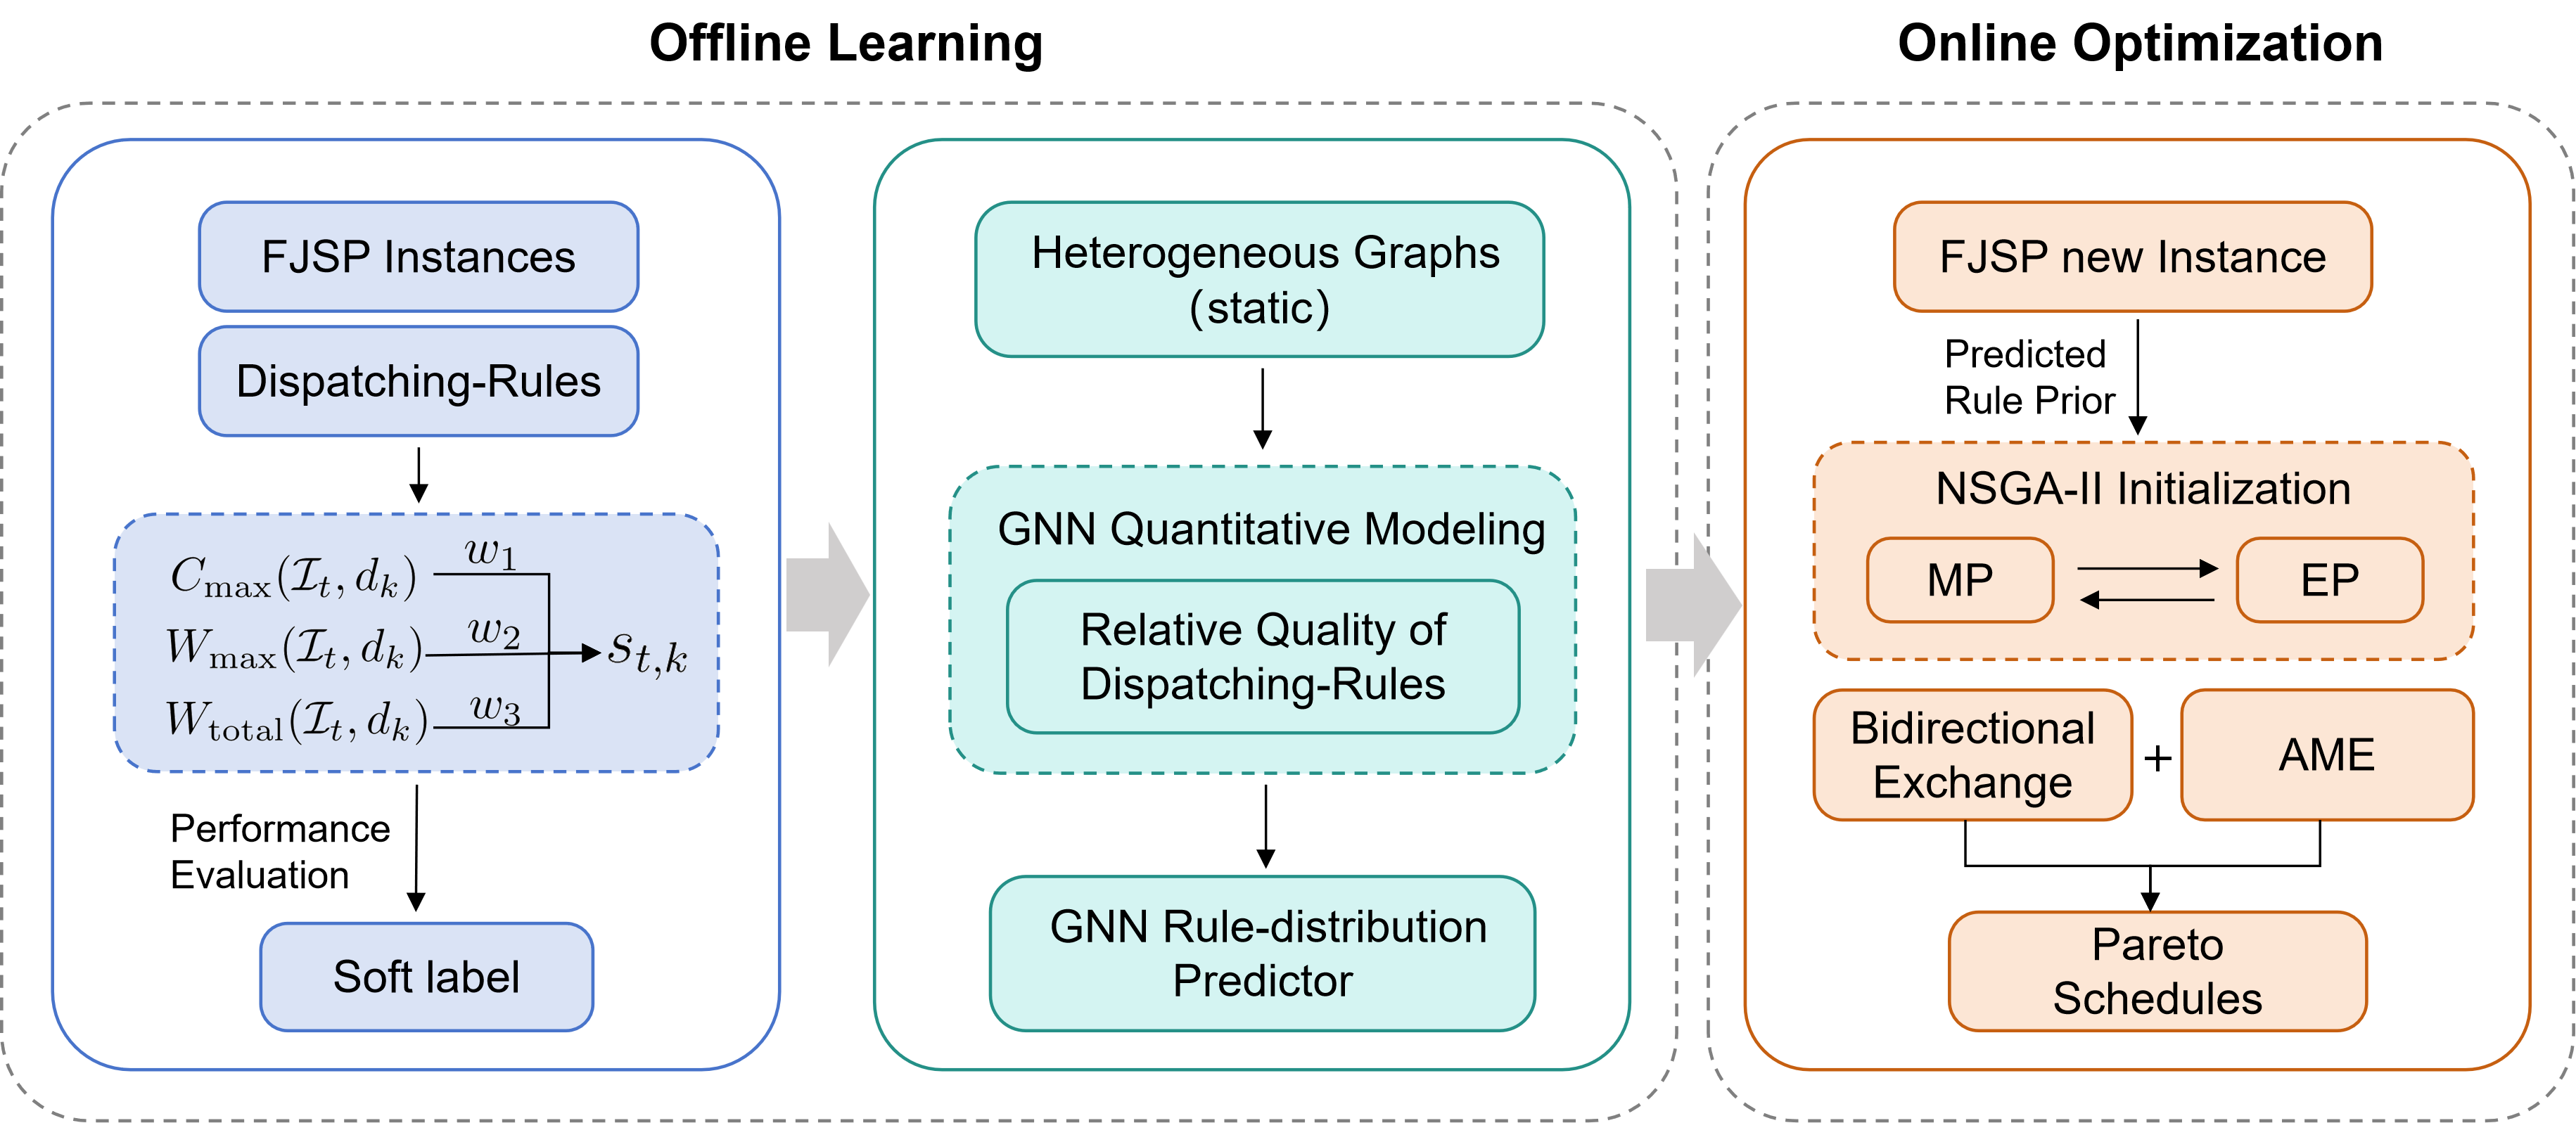
\includegraphics[width=\textwidth]{images/framework.png}
  \caption{Overall architecture of the proposed data-driven heterogeneous dual-population evolutionary framework}
  \label{fig:framework}
\end{figure*}

% 所提 GNN-HDPCEA-AME 框架由离线学习阶段与在线优化阶段构成。
% 在离线阶段，历史或仿真的 FJSP 实例被转换为静态异构析取图。在三个目标下评价一组调度规则组合，并将每个规则组合的多目标性能转换为软概率分布。随后训练一个 GNN 作为图级规则分布回归器。
The proposed GNN-HDPCEA-AME framework consists of an offline learning stage and an online optimization stage, as illustrated in Fig.~\ref{fig:framework}.
In the offline stage, historical or simulated FJSP instances are converted into static heterogeneous disjunctive graphs. A pool of dispatching-rule combinations is evaluated under the three objectives, and the multi-objective performance of each rule combination is transformed into a soft probability distribution. A GNN is then trained as a graph-level rule-distribution regressor.

% 在在线优化阶段，新的 FJSP 实例首先被编码为图并通过训练好的 GNN。所预测的规则分布在双种群 NSGA-II 框架中引导两个异构种群的初始化。
% MP 维持广泛的帕累托前沿覆盖，EP 在有潜力区域附近执行强化搜索。双向交换与自适应混合进化在整个搜索过程中连接两个种群。
In the online optimization stage, a new FJSP instance is first encoded as a graph and passed through the trained GNN. The predicted rule distribution guides the initialization of two heterogeneous populations in a dual-population NSGA-II framework. The MP maintains broad Pareto-front coverage, while the EP performs intensified search around promising regions. Bidirectional exchange and adaptive mixed evolution connect the two populations throughout the search.

% \begin{figure}[t]
%   \centering
%   \fbox{\begin{minipage}{0.92\linewidth}
%       \centering
%       \vspace{0.5em}
%       Offline learning: FJSP instances $\rightarrow$ static heterogeneous graphs $\rightarrow$ GNN rule-distribution predictor.\\[0.5em]
%       Online optimization: new instance $\rightarrow$ predicted rule prior $\rightarrow$ MP/EP initialization $\rightarrow$ bidirectional exchange + AME $\rightarrow$ Pareto schedules.
%       \vspace{0.5em}
%     \end{minipage}}
%   \caption{Overall architecture of the proposed data-driven heterogeneous dual-population evolutionary framework. The placeholder should be replaced by the final framework diagram before submission}
%   \label{fig:framework}
% \end{figure}
% 框架图移到前面了

\subsection{Heterogeneous disjunctive graph representation}\label{subsec:graph}

% % 对于实例 $\mathcal{I}$，改进的异构析取图记为 $\mathcal{G}^{h}=(V,E^d,E^u)$，
% % 其中 $V=V^o\cup V^m\cup{v_s,v_t}$ 包含工序节点、机器节点以及表示全局起始与终止状态的两个虚拟节点。
% % 有向边集 $E^d$ 包括同一作业相邻工序间的先后边、从 $v_s$ 指向首工序的起始边，以及从末工序指向 $v_t$ 的终止边。
% % 无向边集 $E^u$ 将每个工序节点连接到其合格机器节点，从而在不枚举所有机器冲突对的情况下表示机器柔性。
% For an instance $\mathcal{I}$, the improved heterogeneous disjunctive graph is denoted by $\mathcal{G}^{h}=(V,E^d,E^u)$, where $V=V^o\cup V^m\cup\{v_s,v_t\}$ contains operation nodes, machine nodes, and two virtual nodes representing the global start and terminal states.
% The directed edge set $E^d$ includes precedence edges between consecutive operations of the same job, start edges from $v_s$ to the first operations, and terminal edges from the last operations to $v_t$.
% The undirected edge set $E^u$ connects each operation node to its eligible machine nodes, thereby representing machine flexibility without enumerating all machine-conflict pairs.

% % 每个节点由一个四维独热类型向量编码，指示起始节点、工序节点、机器节点或终止节点。
% % 每条边由一个二维特征向量编码，记录关系类型以及在适用时归一化的加工时间属性。工序-机器边携带加工时间信息，先后相关边则编码结构性次序。
% % 该表示是静态的：它在优化开始前描述完整的制造实例，并支持图级监督学习。
% Each node is encoded by a four-dimensional one-hot type vector indicating start node, operation node, machine node, or terminal node.
% Each edge is encoded by a two-dimensional feature vector that records the relation type and the normalized processing-time attribute when applicable. Operation-machine edges carry processing-time information, while precedence-related edges encode structural ordering.
% This representation is static: it describes the complete manufacturing instance before optimization starts and supports graph-level supervised learning.
% -------------------------

% FJSP实例常被表示为析取图，其中机器竞争由析取弧编码，机器约束仅被隐式表达。
% 为显式刻画机器相关信息，异构析取图将机器提取为独立的一类节点，并通过以加工时间为权重的机器-工序弧连接工序与其候选机器。
% 该异构表征主要面向深度强化学习派工中的动态图状态，其节点特征描述随调度推进而变化的状态。
% 由于本文面向的是将完整实例映射为调度规则先验的静态监督学习场景，故从结构微调与特征编码两方面对现有异构析取图加以改进。
An FJSP instance is commonly represented as a disjunctive graph, in which machine competition is encoded by disjunctive arcs and machine constraints remain implicit.
To make machine-related information explicit, a heterogeneous disjunctive graph extracts machines as a separate node type and links each operation to its eligible machines through machine-operation arcs weighted by processing time \cite{song2022flexible}.
This heterogeneous representation is mainly designed for the dynamic graph states used in DRL-based dispatching, where node features describe the evolving scheduling status.
Since this paper targets a static supervised-learning setting that maps a complete instance to dispatching-rule priors, the existing heterogeneous disjunctive graph is improved from two aspects: structural adjustment and feature encoding.

% 改进异构析取图记为 $\mathcal{G}^{hetero}(\mathcal{I})=(\mathcal{V},\mathcal{E}^{dir}\cup\mathcal{E}^{undir},X,E)$。
% 节点集合 $\mathcal{V}=\{v_{start}\}\cup\{v_{end}\}\cup\mathcal{V}_M\cup\mathcal{V}_O$ 将工序节点与机器节点合并入同一集合，并引入两个具全局起止语义的虚拟节点。
% 有向边集 $\mathcal{E}^{dir}=\mathcal{E}_{start}\cup\mathcal{E}_{prec}\cup\mathcal{E}_{end}$ 将原有优先级弧细分为起始边、工序优先级边与终止边；
% 无向边集 $\mathcal{E}^{undir}$ 将每个工序节点连接到其候选机器节点，从而显式表示机器柔性而无需枚举所有同机器工序对。
The improved heterogeneous disjunctive graph is denoted by $\mathcal{G}^{hetero}(\mathcal{I})=(\mathcal{V},\mathcal{E}^{dir}\cup\mathcal{E}^{undir},X,E)$ and is illustrated in Fig.~\ref{fig:heterogeneous_disjunctive_graph_representation}.
The node set $\mathcal{V}=\{v_{start}\}\cup\{v_{end}\}\cup\mathcal{V}_M\cup\mathcal{V}_O$ merges operation nodes $\mathcal{V}_O$ and machine nodes $\mathcal{V}_M$ into one set and adds two virtual nodes $v_{start},v_{end}$ carrying global start and terminal semantics.
The directed edge set $\mathcal{E}^{dir}=\mathcal{E}_{start}\cup\mathcal{E}_{prec}\cup\mathcal{E}_{end}$ refines the precedence arcs into start edges from $v_{start}$ to the first operation of each job, precedence edges between consecutive operations of a job, and terminal edges from the last operation of each job to $v_{end}$.
The undirected edge set $\mathcal{E}^{undir}$ connects each operation node to its eligible machine nodes, so machine flexibility is modeled explicitly without enumerating all machine-conflict pairs.

% 在结构微调基础上设计面向静态图学习的特征编码。
% 节点特征矩阵 $X\in\mathbb{R}^{|\mathcal{V}|\times4}$ 采用节点类型的四维独热编码，区分起始、终止、机器与工序节点，避免依赖调度状态的动态特征，契合静态实例表征。
% 边特征矩阵 $E$ 为每条边赋予二维向量 $[e_{prec},e_{time}]$：$e_{prec}\in\{0,1\}$ 标识是否为有向优先级类边；当边为机器-工序边（$e_{prec}=0$）时，$e_{time}$ 记录加工时间 $p_{ijk}$。
% 该表征在优化开始前完整描述实例，支持图级监督学习。
Building on the structural adjustment, a feature encoding is designed for static graph-level learning.
The node feature matrix $X\in\mathbb{R}^{|\mathcal{V}|\times4}$ adopts a four-dimensional one-hot encoding of the node type, distinguishing start, terminal, machine, and operation nodes, which avoids state-dependent dynamic features and fits the static instance representation.
The edge feature matrix $E$ assigns each edge a two-dimensional vector $[e_{prec},e_{time}]$: $e_{prec}\in\{0,1\}$ indicates whether the edge is a directed precedence-type edge, and $e_{time}$ stores the processing time $p_{ijk}$ when the edge is a machine-operation edge ($e_{prec}=0$).
% 为适配图神经网络输入，该图以边索引张量的形式存储，其中每条无向的工序-机器边由两条方向相反的有向边表示，从而在卷积过程中实现双向的消息传递。
For graph neural network input, the graph is stored as an edge-index tensor in which each undirected operation-machine edge is represented by two opposite directed edges, so that messages can be passed in both directions during convolution.

\begin{figure}[t]
  \centering
  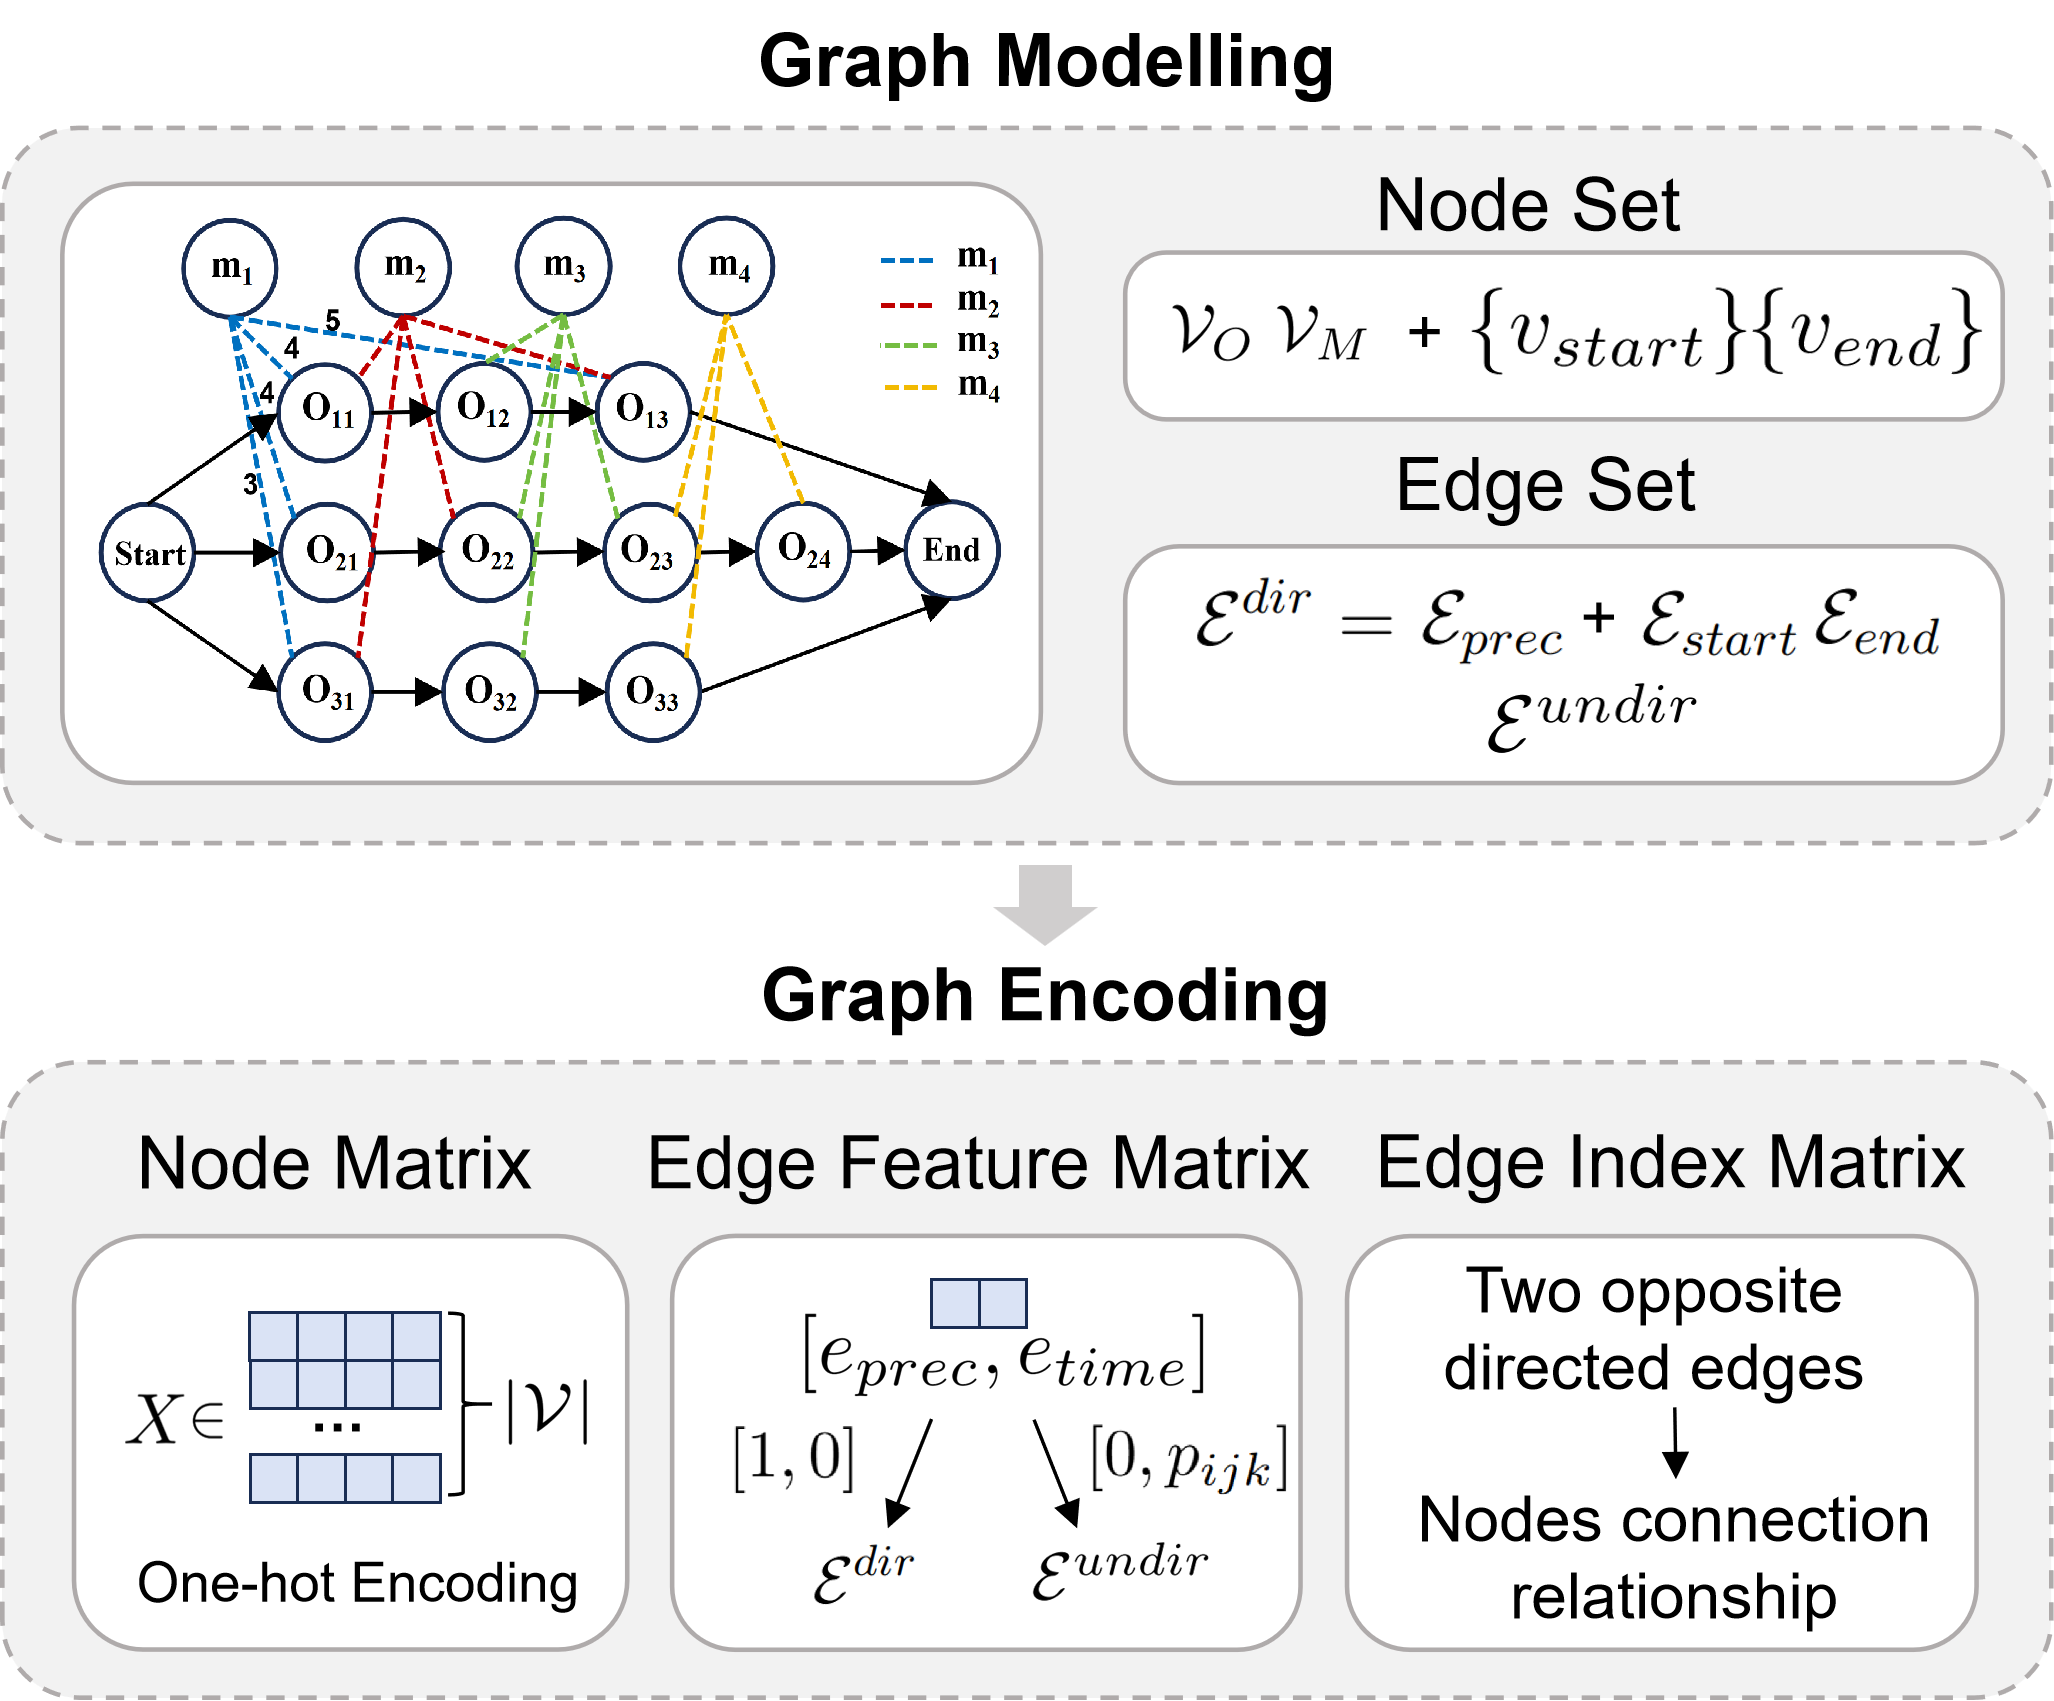
\includegraphics[width=0.92\linewidth]{images/异构析取图表征.png}
  \caption{Heterogeneous disjunctive graph representation}
  \label{fig:heterogeneous_disjunctive_graph_representation}
\end{figure}

\subsection{GNN-based dispatching-rule prior learning}\label{subsec:gnn}

% 令 $\mathbf{h}v^{(l)}$ 为节点 $v$ 在第 $l$ 层的嵌入，$\mathbf{e}{uv}$ 为边 $(u,v)$ 的特征。
% 边条件卷积通过神经网络 $\Theta(\cdot)$ 生成边特定的权重矩阵来更新节点嵌入（式见下）， 
Let $\mathbf{h}_v^{(l)}$ be the embedding of node $v$ at layer $l$ and $\mathbf{e}_{uv}$ be the feature of edge $(u,v)$.
Edge-conditioned convolution updates node embeddings by generating an edge-specific weight matrix through a neural network $\Theta(\cdot)$:
\begin{equation}
  \mathbf{h}_v^{(l+1)} =
  \sigma\left(
  \mathbf{W}^{(l)}\mathbf{h}_v^{(l)}
  + \sum_{u\in\mathcal{N}(v)}
  \Theta^{(l)}(\mathbf{e}_{uv})\mathbf{h}_u^{(l)}
  \right),
\end{equation}
% 其中 $\mathcal{N}(v)$ 表示 $v$ 的邻居，$\sigma(\cdot)$ 为非线性激活函数。该设计使关系类型与加工时间属性能够调制消息传递。
where $\mathcal{N}(v)$ denotes the neighbors of $v$ and $\sigma(\cdot)$ is a nonlinear activation function. This design allows relation types and processing-time attributes to modulate message passing.

% 经过两层边条件卷积后，节点嵌入由全局注意力池化聚合（式见下），其中 $\phi(\cdot)$ 为可学习的门控网络。
% 图表示 $\mathbf{g}$ 被送入全连接回归头，再经 softmax 归一化得到 $\hat{\mathbf{p}}\in[0,1]^K$，其中 $K$ 为保留的调度规则组合数量。
After two edge-conditioned convolution layers, node embeddings are aggregated by global attention pooling:
\begin{equation}
  \mathbf{g}=\sum_{v\in V} a_v\mathbf{h}_v,\qquad
  a_v=\frac{\exp(\phi(\mathbf{h}_v))}{\sum_{u\in V}\exp(\phi(\mathbf{h}_u))},
\end{equation}
where $\phi(\cdot)$ is a learnable gate network.
The graph representation $\mathbf{g}$ is passed to a fully connected regression head followed by softmax normalization to produce $\hat{\mathbf{p}}\in[0,1]^K$, where $K$ is the number of retained dispatching-rule combinations. The overall prior-learning architecture is shown in Fig.~\ref{fig:gnn}.

\begin{figure*}[t]
  \centering
  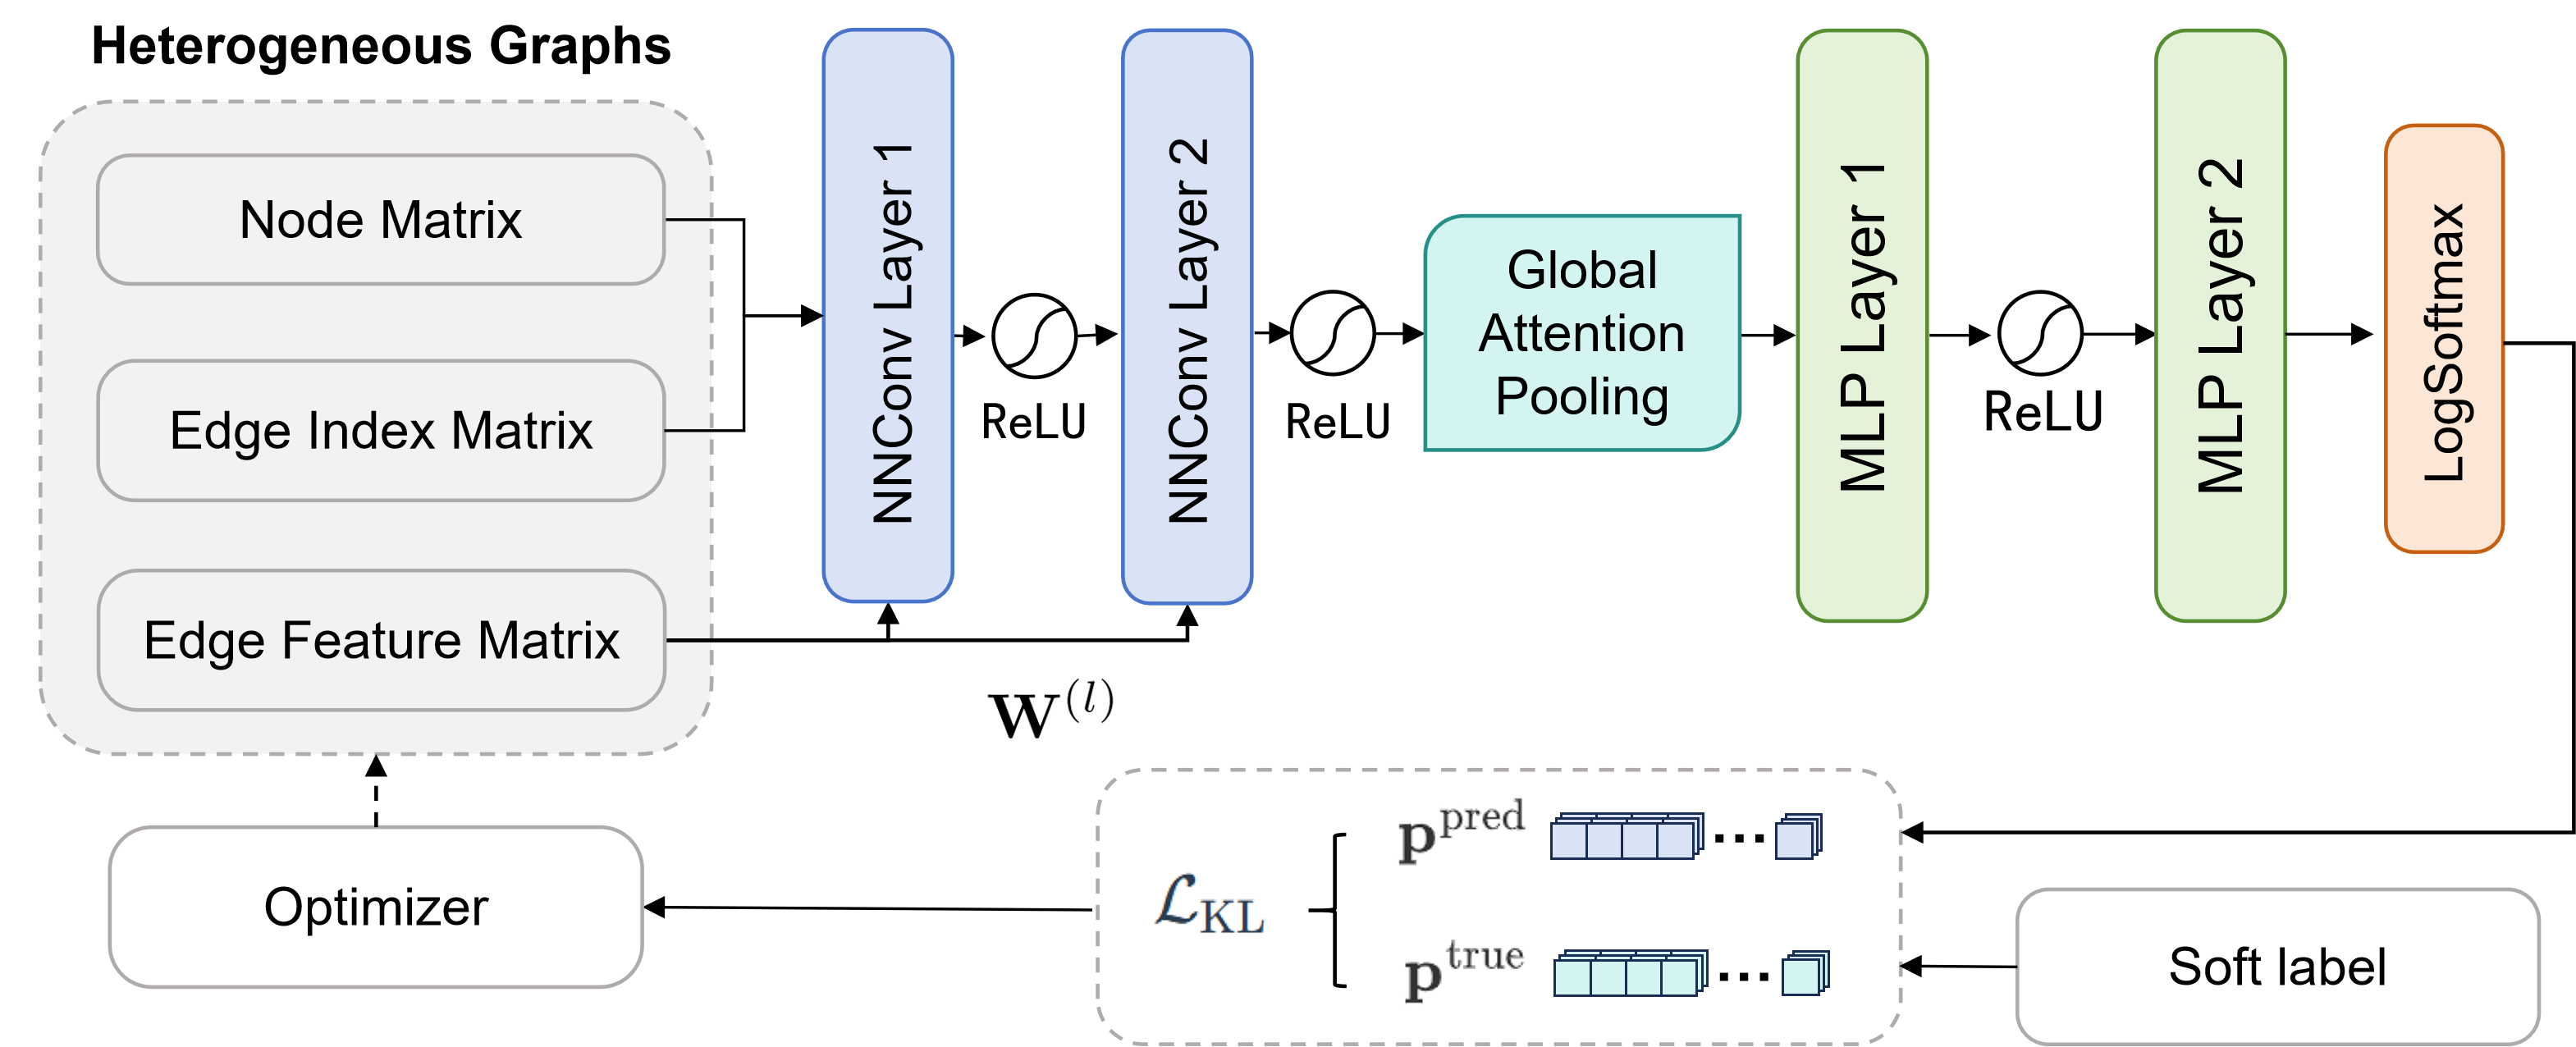
\includegraphics[width=\textwidth]{images/GNN.png}
  \caption{GNN-based dispatching-rule prior learning}
  \label{fig:gnn}
\end{figure*}

\subsection{Multi-objective soft-label construction}\label{subsec:labels}

% 对于训练实例 $\mathcal{I}t$ 与调度规则组合 $d_k$，三个目标值被转换为加权综合分数（式见下），其中 $w_1,w_2,w_3\ge0$ 且 $w_1+w_2+w_3=1$。
% 由于 $W{\mathrm{total}}$ 的量级通常大于 $C_{\max}$ 与 $W_{\max}$，故采用较小的 $w_3$ 以提供隐式的尺度补偿，同时保留其制造含义。
For training instance $\mathcal{I}_t$ and dispatching-rule combination $d_k$, the three objective values are converted into a weighted composite score:
\begin{align}
  s_{t,k} =
   & w_1 C_{\max}(\mathcal{I}_t,d_k)
  + w_2 W_{\max}(\mathcal{I}_t,d_k) \nonumber     \\
   & + w_3 W_{\mathrm{total}}(\mathcal{I}_t,d_k),
\end{align}
where $w_1,w_2,w_3\ge0$ and $w_1+w_2+w_3=1$. Because $W_{\mathrm{total}}$ is usually larger in scale than $C_{\max}$ and $W_{\max}$, a smaller $w_3$ is used to provide implicit scale compensation while preserving its manufacturing meaning.

% 综合分数经对数变换压缩（式见下）。目标软标签通过 softmin 变换获得（式见下）。
% 如此，更优的规则组合获得更高概率，而具竞争力的非最优规则仍保留监督信号。
% GNN 通过最小化 $\mathbf{p}^{multi}$ 与 $\hat{\mathbf{p}}$ 之间的 KL 散度进行训练。
The composite score is compressed by a logarithmic transform:
\begin{equation}
  y_{t,k}^{multi}=\log(s_{t,k}+1).
\end{equation}
The target soft label is obtained by a softmin transform:
\begin{equation}
  p_{t,k}^{multi} =
  \frac{\exp(-y_{t,k}^{multi})}
  {\sum_{l=1}^{K}\exp(-y_{t,l}^{multi})}.
\end{equation}
Thus, better rule combinations receive higher probabilities, while competitive non-best rules still retain supervision signals.
The GNN is trained by minimizing the Kullback--Leibler divergence between $\mathbf{p}^{multi}$ and $\hat{\mathbf{p}}$.

\subsection{Heterogeneous dual-population initialization}\label{subsec:init}

% 训练后的 GNN 输出预测分布 $\hat{\mathbf{p}}$，编码了 $K$ 个调度规则组合在三个加权目标下的相对优劣；
% 由于无论目标个数多少它都仍是 $K$ 维概率向量，多目标偏好被完整承载于 $\hat{\mathbf{p}}$ 中，可被初始化直接利用。
% 为将收敛与多样性解耦，从同一先验出发初始化两个职责互补的种群：MP 负责覆盖帕累托前沿的较广区域，EP 负责在高质量核心区域附近强化搜索。
% 由于两种职责对初始种群提出不同要求，同一先验 $\hat{\mathbf{p}}$ 以两种不同方式被利用。
The trained GNN outputs a predicted distribution $\hat{\mathbf{p}}$ that encodes the relative quality of the $K$ dispatching-rule combinations under the three weighted objectives.
Since it remains a $K$-dimensional probability vector independent of the number of objectives, the multi-objective preference is carried entirely by $\hat{\mathbf{p}}$ and can be consumed directly during initialization.
To decouple convergence from diversity, two populations with complementary roles are initialized from the same prior: the Main Population (MP) is responsible for covering a broad region of the Pareto front, whereas the Exploratory Population (EP) is responsible for intensified search around a high-quality core region.
Because these two roles impose different requirements on the initial population, the shared prior $\hat{\mathbf{p}}$ is exploited in two distinct ways.

% 维持前沿广度要求初始种群具有多样性、分散于多个有潜力的规则组合，而非集中于单一组合。
% 因此 MP 采用一种置信度驱动的利用-探索均衡策略（AdaptiveProbEE），按 $\hat{\mathbf{p}}$ 在各规则组合间分配个体，并依预测置信度调节利用比例。
% 置信度由 $\hat{\mathbf{p}}$ 的归一化熵度量（式见下）。
Maintaining broad front coverage calls for an initial population that is diverse and spread over several promising rule combinations rather than concentrated on one.
The MP is therefore initialized by a confidence-driven exploitation--exploration strategy (denoted AdaptiveProbEE), which allocates individuals across rule combinations in proportion to $\hat{\mathbf{p}}$ and adapts the exploitation ratio to the prediction confidence.
The confidence is measured by the normalized entropy of $\hat{\mathbf{p}}$:
\begin{equation}
  C = 1-\frac{H(\hat{\mathbf{p}})}{\ln K},\qquad
  H(\hat{\mathbf{p}})=-\sum_{k=1}^{K}\hat{p}_k\ln \hat{p}_k.
\end{equation}
% 高 $C$ 表示预测尖锐而可靠，更多个体开发高概率规则；低 $C$ 表示预测不确定，降低利用比例并采样更多探索性组合。
% 由此得到一个嵌入实例先验、又能覆盖较广搜索区域的多样化 MP。
A high $C$ indicates a sharp and reliable prediction, so more individuals exploit the high-probability rules; a low $C$ indicates an uncertain prediction, so the exploitation ratio is reduced and more exploratory combinations are sampled.
This produces a diverse MP that embeds the instance-aware prior while covering a wide region of the search space.
while covering a wide region of the search space; the overall procedure is summarized in Algorithm~\ref{alg:adaptiveprobee}.

\begin{algorithm}[t]
  \caption{AdaptiveProbEE: confidence-driven initialization of MP}
  \label{alg:adaptiveprobee}
  \begin{algorithmic}[1]
    \Require predicted distribution $\hat{\mathbf{p}}$, population size $N_{MP}$,
    confidence threshold $\tau$,
    base ratios and spans $(r^{\mathrm{h}}_{\min},\Delta r^{\mathrm{h}},r^{\mathrm{l}}_{\min},\Delta r^{\mathrm{l}})$,
    perturbation rates $(\rho^{\mathrm{h}}_{\mathrm{exploit}},\rho^{\mathrm{l}}_{\mathrm{exploit}},\rho_{\mathrm{explore}})$
    \Ensure Main population $\mathrm{MP}$
    \State Compute confidence $C \leftarrow 1-H(\hat{\mathbf{p}})/\ln K$
    \If{$C>\tau$} \Comment{high confidence: trust the prior}
    \State $r_{\mathrm{exploit}}\leftarrow r^{\mathrm{h}}_{\min}+\Delta r^{\mathrm{h}}\,(C-\tau)/(1-\tau)$
    \State $\rho_{\mathrm{exploit}}\leftarrow \rho^{\mathrm{h}}_{\mathrm{exploit}}$
    \Else \Comment{low confidence: favor exploration}
    \State $r_{\mathrm{exploit}}\leftarrow r^{\mathrm{l}}_{\min}+\Delta r^{\mathrm{l}}\,C/\tau$
    \State $\rho_{\mathrm{exploit}}\leftarrow \rho^{\mathrm{l}}_{\mathrm{exploit}}$
    \EndIf
    \State $N_{\mathrm{exploit}}\leftarrow\lfloor r_{\mathrm{exploit}}N_{MP}\rfloor$
    \State $N_{\mathrm{explore}}\leftarrow N_{MP}-N_{\mathrm{exploit}}$    \State \textbf{Exploit:} allocate $N_{\mathrm{exploit}}$ individuals to rules in proportion to $\hat{\mathbf{p}}$,
    decode each, and apply mild perturbation $\rho_{\mathrm{exploit}}$
    \State \textbf{Explore:} draw $N_{\mathrm{explore}}$ rules uniformly at random,
    decode each, and apply strong perturbation $\rho_{\mathrm{explore}}$
    \State $\mathrm{MP}\leftarrow$ Shuffle(exploit $\cup$ explore)
    \State \Return $\mathrm{MP}$
  \end{algorithmic}
\end{algorithm}

% 在核心区域附近强化搜索则要求一个聚焦的种子种群，定位于该实例预测的最优折衷附近。
% 因此 EP 由预测概率最高的单一规则组合 ($k^*=\arg\max_k \hat p_k$) 生成近似同质的种群，
% 除首个个体外，其余个体在工序序列与机器选择编码上施加轻微扰动以避免完全重复。
The opposite role, intensifying search around a high-quality core region, calls for a focused seed population located near the best compromise predicted for the instance. The EP is therefore initialized from the single rule combination with the highest predicted probability ($k^{*}=\arg\max_k \hat{p}_k$, denoted BestSingleRule), forming a near-homogeneous population in which every individual except the first is slightly perturbed in its operation-sequence and machine-selection encodings to avoid exact duplication.
% 由于预测概率最高的规则通常对应该实例上综合性能最优的折衷方案，这一聚焦初始化为 EP 提供了一个高质量核心，便于其进行深度邻域开发。
Since the top-predicted rule usually corresponds to the best overall multi-objective compromise for the instance, this focused initialization provides the EP with a high-quality core from which to perform deep neighborhood exploitation.

\begin{algorithm}[t]
  \caption{GNN-HDPCEA-AME for multi-objective FJSP}
  \label{alg:gnn_hdpcea}
  \begin{algorithmic}[1]
    \Require FJSP instance $\mathcal{I}$, trained GNN predictor, population sizes $N_{MP},N_{EP}$, maximum generation $G$
    \Ensure Approximate Pareto schedule set $\mathcal{A}$
    \State Encode $\mathcal{I}$ as static heterogeneous graph $\mathcal{G}^{h}$
    \State Predict rule distribution $\hat{\mathbf{p}} \leftarrow \mathrm{GNN}(\mathcal{G}^{h})$
    \State Compute prediction confidence $C$ from $\hat{\mathbf{p}}$
    \State Initialize MP by AdaptiveProbEE using $\hat{\mathbf{p}}$
    \State Initialize EP by BestSingleRule using $\hat{\mathbf{p}}$
    \For{$g=1$ to $G$}
    \State Generate MP offspring using NSGA-II variation and decoding
    \State Update MP by non-dominated sorting and crowding distance
    \State Generate EP offspring by adaptive mixed evolution
    \State Update EP by non-dominated sorting and crowding distance
    \If{$g$ is an exchange generation}
    \State Inject EP elites into MP
    \State Inject MP diversity anchors into EP
    \EndIf
    \EndFor
    \State $\mathcal{A}\leftarrow$ non-dominated solutions in MP $\cup$ EP
    \State \Return $\mathcal{A}$
  \end{algorithmic}
\end{algorithm}


\subsection{Bidirectional population exchange and adaptive mixed evolution}\label{subsec:exchange_ame}

% 若两个种群孤立进化，其互补优势将无法共享：MP 缺少 EP 深度开发所发现的接近前沿的解，
% 而受同质化初始化限制的 EP 也难以扩展到更多样的区域。为此引入双向交换，使两个种群周期性地相互增强。
If the two populations evolved in isolation, their complementary strengths could not be shared: the MP would lack the near-front solutions discovered by the EP's exploitation, while the EP, constrained by its homogeneous initialization, would struggle to reach more diverse regions.
A bidirectional exchange is therefore introduced so that the two populations periodically reinforce each other.

% 每个交换周期，将 EP 中排名前 10% 的精英个体注入 MP。
% 这些个体从 EP 的最优非支配前沿中选出，并替换 MP 中低优先级（最差层）的个体。
% 该方向有助于 MP 吸收 EP 局部开发所发现的高质量解。
Every exchange period, the top 10\% elite individuals from EP are injected into MP.
These individuals are selected from the best non-dominated fronts of EP and replace individuals in the worst front of MP.
This direction helps MP absorb high-quality solutions discovered by EP's local exploitation.
% 在相反方向上，将 MP 中拥挤距离较大的 5% 个体作为多样性锚点注入 EP。
% 这些个体通常位于当前前沿的稀疏区域，为 EP 提供新的可探索邻域。
% 交换比例是非对称的，因为 EP 向 MP 贡献偏开发的精英，而 MP 只需提供少量多样性锚点以重定向 EP。
In the opposite direction, 5\% of MP individuals with large crowding distances are injected into EP as diversity anchors.
These individuals usually lie in sparse regions of the current front and provide new neighborhoods for EP to explore.
The exchange ratio is asymmetric because the MP is the primary source of the final Pareto front and benefits from EP elites, whereas the EP relies mainly on its own evolution and needs only a few diverse anchors to redirect its search.

% 由于 EP 由单一规则组合初始化，个体高度相似，标准交叉变异将失效：近乎相同的父代之间的交叉难以产生有意义的新解。
% 因此 EP 需要一种不依赖父代差异的子代生成机制。
% 自适应混合演化（AME）从三个来源生成 EP 后代以满足该需求。
Because the EP is initialized from a single rule combination, its individuals are highly similar, and standard crossover would be ineffective, since recombining near-identical parents rarely yields meaningful new solutions.
The EP therefore requires an offspring-generation mechanism that does not rely on parent diversity.
Adaptive mixed evolution (AME) meets this need by generating EP offspring from three sources: random injection, neighborhoods of EP elites, and neighborhoods of MP front individuals.
% 三个来源比例随进化进程 $g/G$ 分段设定，如公式所示；MP 前沿邻域始终为最大来源且随进程上升。
The source ratios $(\alpha_{\mathrm{rand}},\alpha_{\mathrm{ep}},\alpha_{\mathrm{mp}})$ are set piecewise according to the evolutionary progress $g/G$, as summarized in Table~\ref{tab:ame_ratio}, with $\alpha_{\mathrm{mp}}=1-\alpha_{\mathrm{rand}}-\alpha_{\mathrm{ep}}$. The numbers of offspring drawn from the three sources are
\begin{equation}
  \label{eq:ame_ratio}
  \begin{aligned}
    n_{\mathrm{rand}} & =\max(1,\lfloor N_{EP}\alpha_{\mathrm{rand}}\rfloor), \\
    n_{\mathrm{ep}}   & =\max(1,\lfloor N_{EP}\alpha_{\mathrm{ep}}\rfloor),   \\
    n_{\mathrm{mp}}   & =N_{EP}-n_{\mathrm{rand}}-n_{\mathrm{ep}}.
  \end{aligned}
\end{equation}
% 随进化推进，随机注入与 EP 精英邻域比例下降、MP 前沿邻域比例上升：
% 早期较多的随机注入与 EP 精英扰动用于打破初始同质化，后期将子代更多移向 MP 前沿以对已趋稳定的高多样性前沿做精细邻域挖掘。
As the search proceeds, the shares of random injection and EP-elite neighborhoods decrease while that of the MP-front neighborhoods increases.
Early generations rely more on random injection and EP-elite perturbation to break the initial homogeneity of EP, whereas later generations shift more offspring toward the MP front to refine the search around its stabilized, diverse front.

% 六种邻域算子覆盖两个编码维度：三种作用于工序序列且扰动依次增强（相邻交换、插入移位、片段逆序），
% 两种作用于机器选择（单工序随机重指派，以及缓解最高负载机器的瓶颈机器批量重指派），另有一种同时扰动两个维度。
% 每个子代等概率随机选取一种算子，使 EP 能够同时搜索排序与机器路由决策
The six neighborhood operators cover both encoding dimensions: three act on the operation sequence with increasing perturbation strength (adjacent swap, insertion, and segment reversal), two act on machine selection (a random single-operation reassignment and a bottleneck-machine batch reassignment that relieves the most-loaded machine), and one perturbs both dimensions jointly.
One operator is selected at random for each offspring, enabling the EP to search sequencing and routing decisions simultaneously.

The overall procedure is illustrated in Fig.~\ref{fig:Exchange_AME}: the MP and EP evolve in parallel through NSGA-II variation and AME, respectively, periodically reinforce each other through the bidirectional exchange, and are finally merged and non-dominated-sorted to produce the output Pareto schedules.
\begin{figure*}[t]
  \centering
  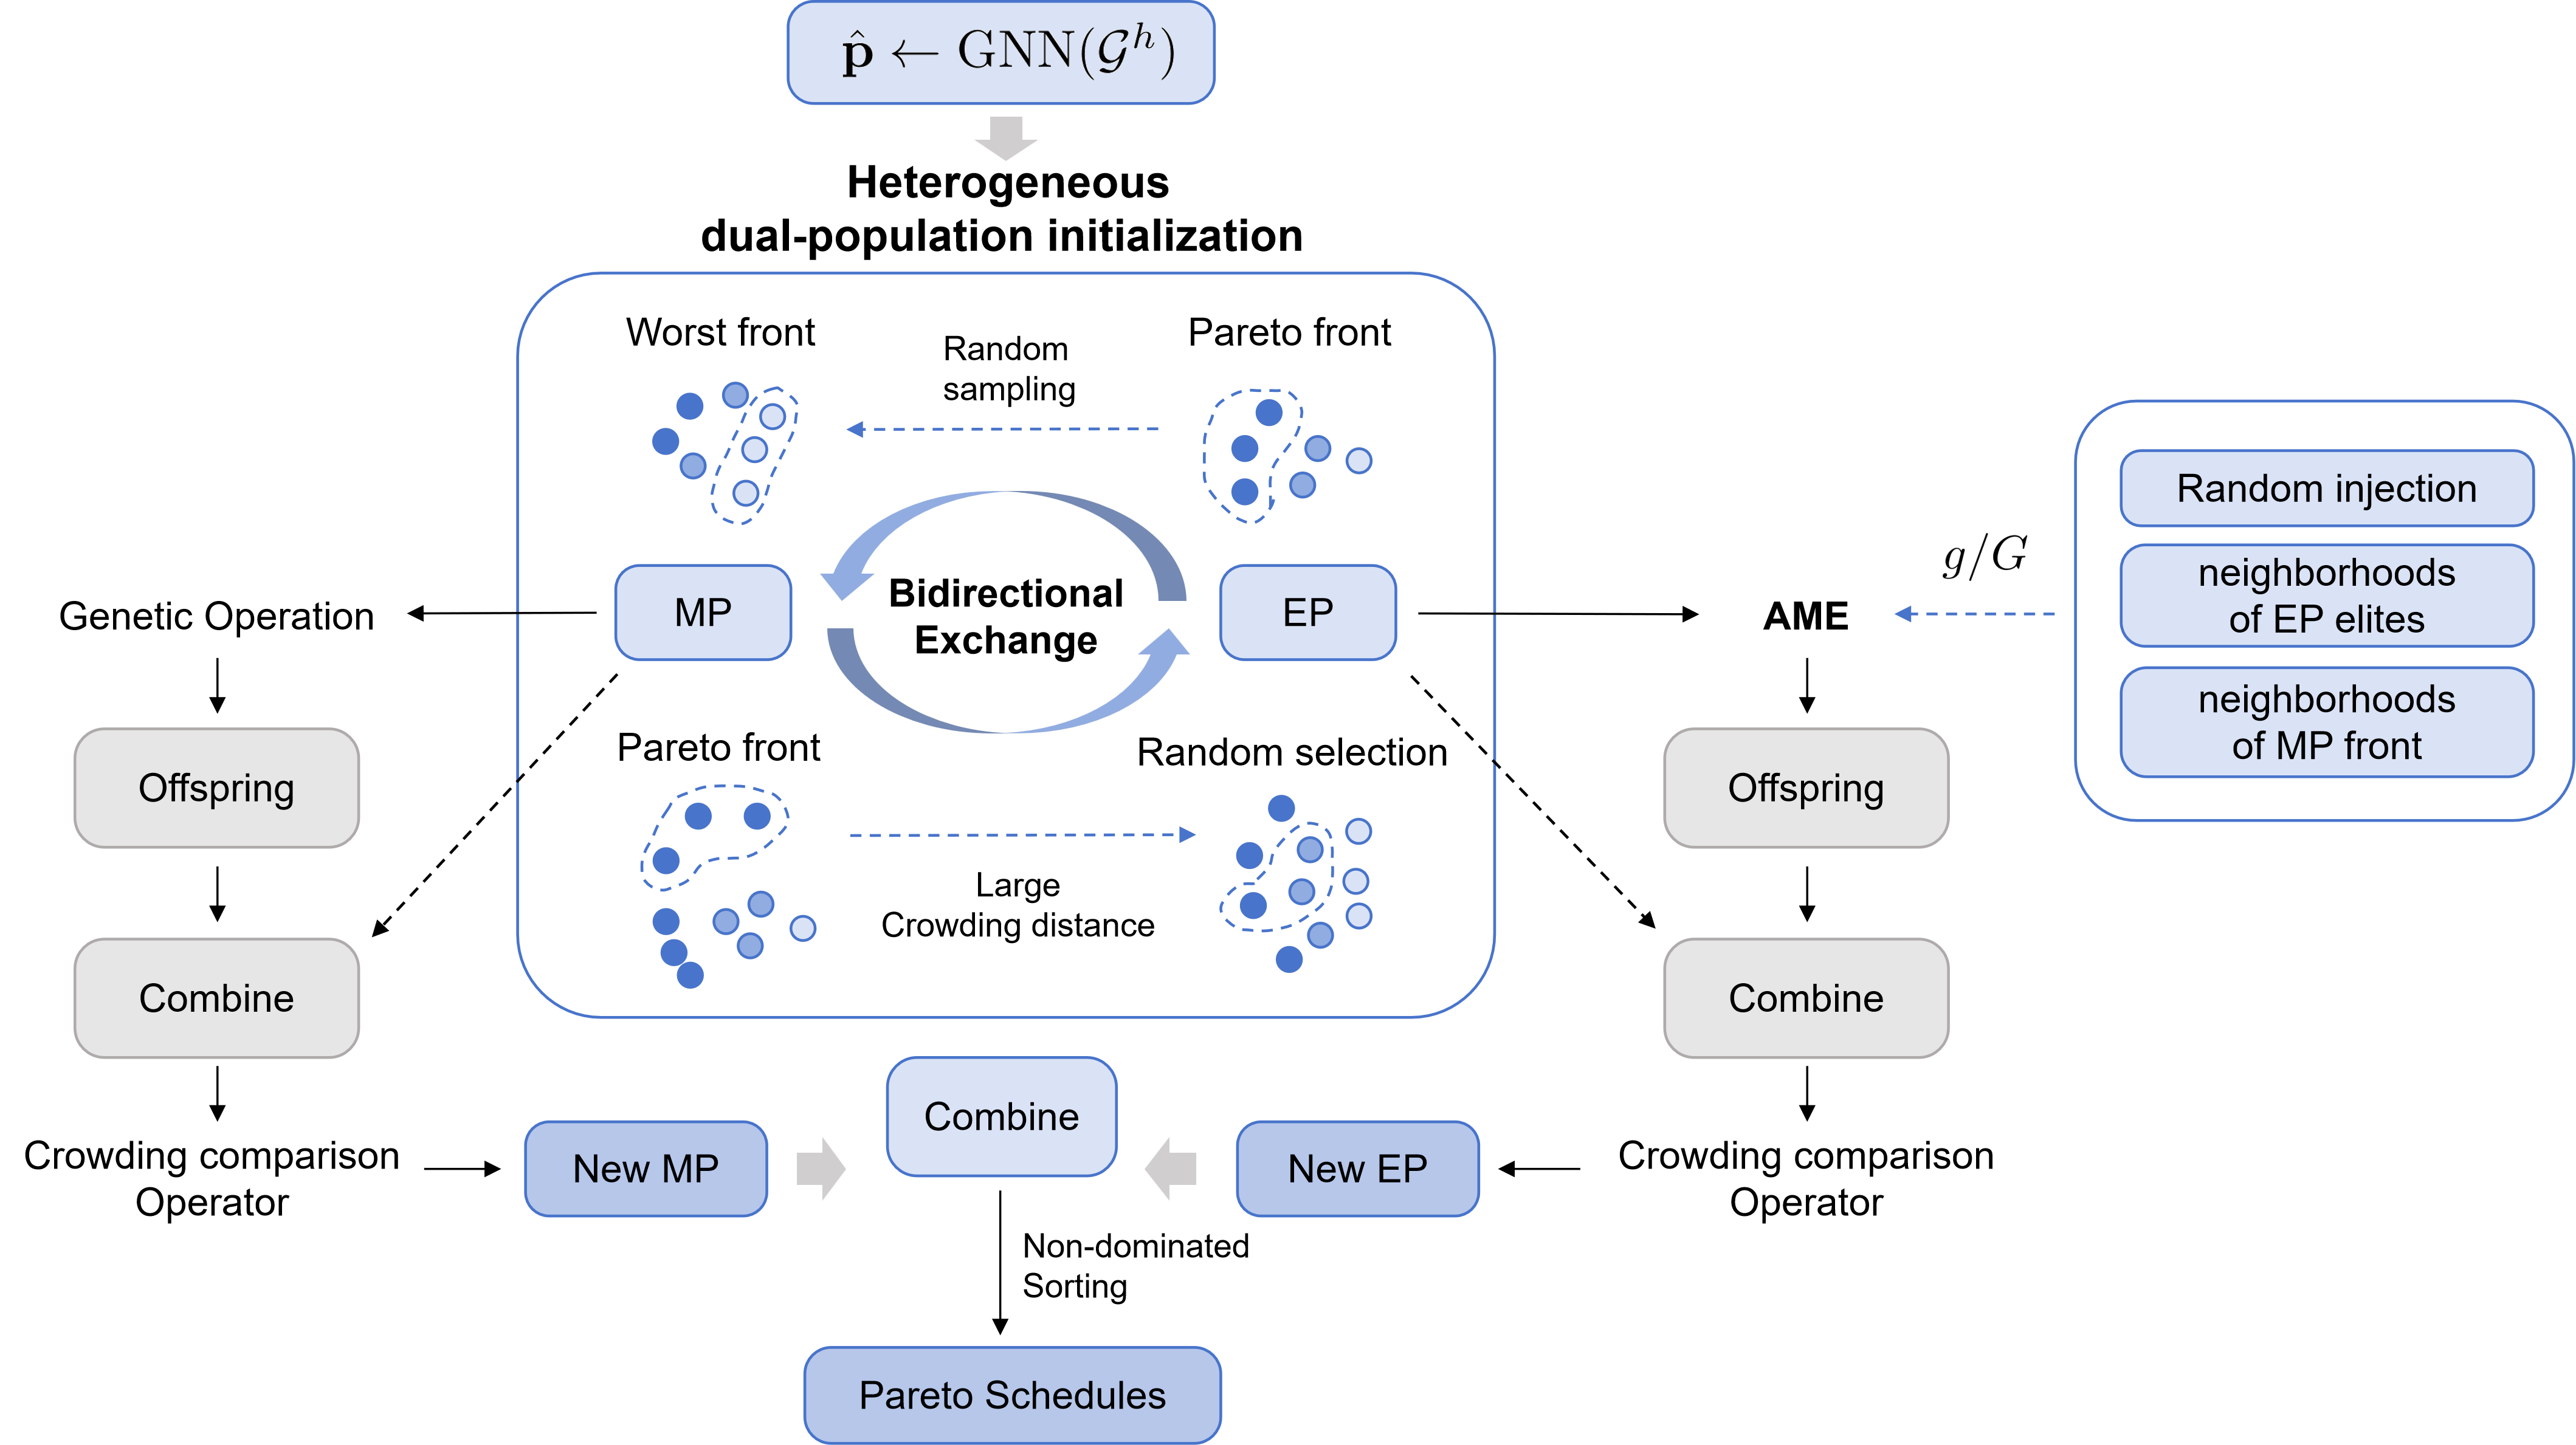
\includegraphics[width=\textwidth]{images/Exchange_AME.png}
  \caption{Workflow of Bidirectional population exchange and Adaptive Mixed Evolution (AME) of the EP}
  \label{fig:Exchange_AME}
\end{figure*}

\begin{table}[t]
  \caption{Adaptive source ratios of AME by evolutionary stage}
  \label{tab:ame_ratio}
  \centering
  \begin{tabular}{lccc}
    \toprule
    Stage $g/G$ & $\alpha_{\mathrm{rand}}$ & $\alpha_{\mathrm{ep}}$ & $\alpha_{\mathrm{mp}}$ \\
    \midrule
    $[0,0.4)$   & 0.15                     & 0.30                   & 0.55                   \\
    $[0.4,0.8)$ & 0.08                     & 0.25                   & 0.67                   \\
    $[0.8,1]$   & 0.05                     & 0.20                   & 0.75                   \\
    \bottomrule
  \end{tabular}
\end{table}
% \begin{table*}[t]
%   \caption{Datasets and main experimental settings}
%   \label{tab:datasets}
%   \centering
%   \begin{tabularx}{0.88\textwidth}{lXXX}
%     \toprule
%     Dataset       & Purpose                 & Scale                 & Notes                        \\
%     \midrule
%     Synthetic set & GNN training/evaluation & 1000 instances        & Jobs 5--20, machines 4--10   \\
%     Brandimarte   & Public benchmark        & Mk01--Mk10            & Standard FJSP instances      \\
%     BehnkeGeiger  & Public benchmark        & Work-center instances & Used for generalization test \\
%     \bottomrule
%   \end{tabularx}
% \end{table*}


\section{Experimental design}\label{sec:experimental_design}

\subsection{Datasets and implementation}\label{subsec:datasets}
% GNN 预测器在由随机制造参数生成的合成 FJSP 实例集上训练与验证。
% 作业数从 ${5,10,15,20}$ 中采样，机器数从 ${4,6,8,10}$ 中采样，柔性比设为 0.5，加工时间从 $[1,100]$ 中采样。
% 共生成 1000 个实例，并通过分层抽样划分为训练集与验证集。
The GNN predictor was trained and validated on a synthetic FJSP instance set generated by randomized manufacturing parameters.
The number of jobs was sampled from $\{5,10,15,20\}$, the number of machines from $\{4,6,8,10\}$, the flexibility ratio was set to 0.5, and processing times were sampled from $[1,100]$.
A total of 1000 instances were generated and split into training and validation sets by stratified sampling.

% 公开基准评价使用  BehnkeGeiger 实例。
% Hurink-rdata 实例未用于多目标评价，因为在当前目标定义下，其加工时间结构导致 $W_{\mathrm{total}}$ 目标上的区分度有限。
Public benchmark evaluation used BehnkeGeiger instances \cite{behnke2012test}.
Hurink-rdata instances \cite{hurink1994tabu} were not used in the multi-objective evaluation because their processing-time structure leads to limited discrimination in the $W_{\mathrm{total}}$ objective under the current objective definition.

% 派工规则池由作业排序规则与机器选择规则构成,候选规则取自 Lei 等人\cite{lei2022multi};在过滤低频规则组合后,保留五个组合作为 GNN 输出类别：FIFO+SPT、MOPNR+SPT、MOPNR+EET、MWKR+SPT 与 MWKR+EET。
The dispatching-rule pool was constructed from job-sequencing rules and machine-selection rules adopted from Lei et al.~\cite{lei2022multi}. After filtering low-frequency rule combinations, five combinations were retained as GNN output classes: FIFO+SPT, MOPNR+SPT, MOPNR+EET, MWKR+SPT, and MWKR+EET.
% 对每个实例，每个候选规则组合都用于初始化一个标准 NSGA-II；将其在 $R$ 次运行上得到的三目标平均性能通过第~\ref{subsec:labels}节的构造映射为软标签，从而得到（实例图，软标签）训练样本对；
% 实验所用的评估参数、AdaptiveProbEE 初始化参数与 GNN 训练超参统一见表\ref{tab:params};后者按各项作用设定、跨所有基准固定,不在公共测试集上重新调参
For each instance, every candidate rule combination seeds a standard NSGA-II, and the averaged three-objective performance over $R$ runs is mapped to a soft label via the construction of Section~\ref{subsec:labels}, giving the (instance graph, soft-label) training pairs.
The parameter, initialization, and GNN-training settings used in the experiments are summarized in Table~\ref{tab:params}; the AdaptiveProbEE values are set according to the role of each term rather than per-instance tuning, and are kept fixed across all benchmarks without re-tuning on the public test sets.
% 所有实验在基于 Linux 的容器环境中进行。服务器配备两块 Intel Xeon Gold 6248R CPU、251 GB 内存以及两块 NVIDIA RTX 3090 GPU。
% 实现使用 Python 3.8.6 与 PyTorch 1.7.1，CUDA 版本为 11.0。每个随机算法独立重复运行，报告平均结果。
All experiments were conducted in a Linux-based container environment. The server was equipped with two Intel Xeon Gold 6248R CPUs, 251 GB memory, and two NVIDIA RTX 3090 GPUs. The implementation used Python 3.8.6 and PyTorch 1.7.1 with CUDA 11.0. Each stochastic algorithm was independently repeated, and average results are reported.

\begin{table}[t]
  \caption{Parameter and hyperparameter settings used in the experiments}
  \label{tab:params}
  \centering
  \begin{tabular}{lcc}
    \toprule
    Parameter                    & Symbol                                 & Value \\
    \midrule
    \multicolumn{3}{l}{\textit{Performance-label evaluation (offline NSGA-II)}}   \\
    Population size              & $N_{pop}$                              & 100   \\
    Maximum generations          & $G$                                    & 50    \\
    Independent runs             & $R$                                    & 10    \\
    Crossover probability        & $p_c$                                  & 0.8   \\
    Mutation probability         & $p_m$                                  & 0.1   \\
    \addlinespace
    \multicolumn{3}{l}{\textit{AdaptiveProbEE initialization}}                    \\
    Confidence threshold         & $\tau$                                 & 0.3   \\
    High-conf.\ base ratio       & $r^{\mathrm{h}}_{\min}$                & 0.70  \\
    High-conf.\ ratio span       & $\Delta r^{\mathrm{h}}$                & 0.20  \\
    Low-conf.\ base ratio        & $r^{\mathrm{l}}_{\min}$                & 0.40  \\
    Low-conf.\ ratio span        & $\Delta r^{\mathrm{l}}$                & 0.30  \\
    High-conf.\ exploit perturb. & $\rho^{\mathrm{h}}_{\mathrm{exploit}}$ & 0.10  \\
    Low-conf.\ exploit perturb.  & $\rho^{\mathrm{l}}_{\mathrm{exploit}}$ & 0.25  \\
    Explore perturbation         & $\rho_{\mathrm{explore}}$              & 0.30  \\
    \addlinespace
    \multicolumn{3}{l}{\textit{GNN training}}                                     \\
    Hidden dimension             & $d_h$                                  & 64    \\
    Training epochs              & $epoch$                                & 100   \\
    Initial learning rate        & $\eta$                                 & 0.001 \\
    Gradient-accum.\ steps       & $N_{batch}$                            & 32    \\
    Dropout rate                 & $p_{drop}$                             & 0.5   \\
    LR-decay patience            & $patience$                             & 8     \\
    LR decay factor              & $\gamma_{lr}$                          & 0.5   \\
    Train split ratio            & $r_{train}$                            & 0.8   \\
    \bottomrule
  \end{tabular}
\end{table}

\subsection{Evaluation metrics}\label{subsec:metrics}

% % 多目标解质量采用四项互补指标度量。
% 超体积（HV）同时反映收敛性与覆盖度，当前沿在目标空间中支配的体积越大其值越大。
% 反世代距离（IGD）以所有对比方法的非支配解合并得到的参考前沿为基准，计算参考前沿中各点到所求前沿的平均距离，值越小表示逼近越好。
% 间距 $\Delta$ 刻画前沿上解分布的均匀性，间距方差 $\Delta_v$ 度量该分布在重复运行间的稳定性，二者均越小越好。
% 这四项指标共同覆盖收敛性、接近度、分布均匀性与稳定性。
The quality of the multi-objective solutions is measured by four complementary metrics.
Hypervolume (HV) reflects both convergence and coverage and is larger when the front dominates a larger objective-space volume. Its reference point is set to $\mathbf{r}=1.1\cdot(\max_i f_1^{(i)},\,\max_i f_2^{(i)},\,\max_i f_3^{(i)})$, i.e.\ $1.1\times$ the per-objective maxima taken over the merged non-dominated solutions of all methods compared in the same experiment.
The inverted generational distance (IGD) is computed against a reference front merged from the non-dominated solutions of all compared methods, by averaging the distance from each point of this reference front to the obtained front; smaller values indicate a closer approximation.
Because both the HV reference point $\mathbf{r}$ and the IGD reference front are built from the union of the methods compared within a given experiment, a table that includes methods with more extended fronts pushes $\mathbf{r}$ outward and thereby inflates the HV magnitudes of \emph{all} entries in that table. Consequently the absolute HV and IGD values are comparable within each table but not directly across tables that correspond to different method sets; this effect is made explicit in Section~\ref{subsec:rq3}.
Spacing $\Delta$ characterizes the uniformity of the solution distribution along the front, and the spacing variance $\Delta_v$ measures the stability of this distribution across repeated runs; smaller values of both are preferable.
Together they cover convergence, proximity, distribution uniformity, and stability.

% GNN 的预测质量从三个维度考察，每个维度选取一项代表性指标。
% 分布拟合质量由 Jensen--Shannon（JS）散度、余弦相似度与 Brier 分数评估，三者共同从形状与量级上刻画预测分布与目标软标签的接近程度。
% 优势规则集合匹配由 Top-3 匹配率（Top-3 Match）评估，衡量最具竞争力的规则组合是否被纳入预测的前几位。
% 最优规则命中由 Top-3 准确率（Top-3 Accuracy）评估，衡量真正最优的规则组合是否落入预测的前几个候选之中。
% 这三个维度分别反映整体分布保真度、竞争规则的覆盖程度，以及识别单一最优规则的可靠性。
The prediction quality of the GNN is examined from three aspects, each with one representative metric.
Distribution-fitting quality is assessed by the Jensen--Shannon (JS) divergence, cosine similarity, and Brier score, which jointly quantify how closely the predicted distribution matches the target soft label in shape and magnitude.
Advantage-rule-set matching is assessed by the Top-3 match rate (Top-3 Match), which measures whether the most competitive rule combinations are captured among the top predictions.
Best-rule hit is assessed by the Top-3 accuracy (Top-3 Accuracy), which measures whether the truly best rule combination falls within the top predicted candidates.
These three aspects respectively reflect overall distribution fidelity, the coverage of competitive rules, and the reliability of identifying the single best rule.

% \subsection{Dispatching-rule pool and compared methods}\label{subsec:baselines}
% % GNN 使用 64 维隐藏层、两层 NNConv、0.5 的 dropout、0.001 的学习率、在 32 个实例上进行梯度累积，并训练 100 个 epoch。
% The GNN used a hidden dimension of 64, two NNConv layers, dropout of 0.5, learning rate of 0.001, gradient accumulation over 32 instances, and 100 training epochs.

% % 完整框架与四组基线进行比较：随机初始化的单种群 NSGA-II、AdaptiveProbEE 初始化的单种群 NSGA-II、不含 AME 的 GNN-HDPCEA-AEE-BSR，以及同质双种群变体。
% % 这些基线分别隔离了所学先验初始化、异构种群角色、双向交换与 AME 的作用。
% The full framework was compared with four groups of baselines: random-initialized single-population NSGA-II, AdaptiveProbEE-initialized single-population NSGA-II, GNN-HDPCEA-AEE-BSR without AME, and homogeneous dual-population variants.
% These baselines isolate the effect of learned prior initialization, heterogeneous population roles, bidirectional exchange, and AME.

% \begin{table}[t]
%   \caption{Compared methods}
%   \label{tab:baselines}
%   \centering
%   \begin{tabularx}{\linewidth}{lX}
%     \toprule
%     Method                               & Purpose                                                 \\
%     \midrule
%     Random NSGA-II                       & Basic single-population evolutionary baseline           \\
%     AdaptiveProbEE NSGA-II               & Single-population baseline using learned initialization \\
%     GNN-HDPCEA-AEE-BSR                   & Dual-population baseline without AME                    \\
%     Homogeneous dual-population variants & Test whether role heterogeneity matters                 \\
%     GNN-HDPCEA-AME                       & Proposed full framework                                 \\
%     \bottomrule
%   \end{tabularx}
% \end{table}

% \subsection{Evaluation metrics}\label{subsec:metrics}
% % 采用四个指标评价帕累托前沿质量。
% % 超体积（HV）相对于参考点度量被支配的体积，当前沿具有更好的收敛性与覆盖度时其值更大。
% % IGD 计算从参考前沿（由所有对比方法的非支配解合并得到）到所得前沿的平均距离，值越小表示越接近。
% % 间距 $\Delta$ 度量前沿解之间最近邻距离的标准差（式见下）。
% % 间距方差 $\Delta_v$ 是 $\Delta$ 在重复运行间的平均绝对偏差，反映分布稳定性。
% Four metrics were used to evaluate Pareto-front quality.
% Hypervolume (HV) measures the dominated volume with respect to a reference point and is larger when the front has better convergence and coverage.
% IGD computes the average distance from a reference front, obtained by merging the non-dominated solutions of all compared methods, to the obtained front; smaller values indicate better proximity.
% Spacing $\Delta$ measures the standard deviation of nearest-neighbor distances among front solutions:
% \begin{equation}
%   \Delta=\sqrt{\frac{1}{|\mathcal{A}|-1}\sum_{\mathbf{x}\in\mathcal{A}}(d(\mathbf{x})-\bar{d})^2}.
% \end{equation}
% The spacing variance $\Delta_v$ is the average absolute deviation of $\Delta$ across repeated runs and reflects distribution stability.

% % GNN 预测器通过 Jensen–Shannon 散度、余弦相似度、Brier 分数及 top-$k$ 匹配指标进行评价。
% % 这些指标评估预测分布是否拟合目标软标签，以及是否捕捉到具有优势的调度规则组合集合。
% The GNN predictor was evaluated by Jensen--Shannon divergence, cosine similarity, Brier score, and top-$k$ matching metrics.
% These metrics assess whether the predicted distribution fits the target soft label and captures the set of advantageous dispatching-rule combinations.

% \section{Results and discussion}\label{sec:results}

% \subsection{Overall multi-objective scheduling performance}\label{subsec:overall_results}

% Table~\ref{tab:overall_results} summarizes the main multi-objective results on the custom validation set. The proposed GNN-HDPCEA-AME achieved the best values on all four metrics. HV reached $5.06\times10^7$, IGD was 16.8174, $\Delta$ was 3.5044, and $\Delta_v$ was 1.3948. Compared with GNN-HDPCEA-AEE-BSR without AME, the full framework improved HV by 13.2\%. Compared with AdaptiveProbEE single-population NSGA-II and random NSGA-II, HV improved by 23.5\% and 66.0\%, respectively. These results indicate that the learned initialization, heterogeneous dual-population structure, and AME jointly improve Pareto-front quality.

% \begin{table*}[t]
%   \caption{Overall performance on the custom validation set}
%   \label{tab:overall_results}
%   \centering
%   \begin{tabular}{lrrrr}
%     \toprule
%     Method                 & HV $\uparrow$               & IGD $\downarrow$ & $\Delta \downarrow$ & $\Delta_v \downarrow$ \\
%     \midrule
%     Random NSGA-II         & $3.05{\times}10^7$          & --                 & --                  & --                    \\
%     AdaptiveProbEE NSGA-II & $4.10{\times}10^7$          & --                 & --                  & --                    \\
%     GNN-HDPCEA-AEE-BSR     & $4.47{\times}10^7$          & --                 & 5.535               & 2.030                 \\
%     GNN-HDPCEA-AME         & $\mathbf{5.06{\times}10^7}$ & $\mathbf{16.8174}$ & $\mathbf{3.5044}$   & $\mathbf{1.3948}$     \\
%     \bottomrule
%   \end{tabular}
% \end{table*}

% On BehnkeGeiger instances, the proposed framework also maintained stable advantages under both 200/100 and 400/200 population/generation configurations. Under the 200/100 configuration, HV reached $3.61\times10^6$, exceeding GNN-HDPCEA-AEE-BSR by approximately 2.8\% and the random baseline by 78.7\%. Although the relative gain over the dual-population baseline was smaller on this public set than on the custom set, the results still suggest that AME improves distribution stability without substantially sacrificing solution quality.

% \subsection{Effectiveness of graph-based prior learning}\label{subsec:gnn_results}

% The proposed NNConv-Attention predictor was compared with NNConv-Mean, NNConv-SAG, NNConv-Set2Set, and NNConv-Deep-Attention. All models used the same input instances and soft labels and differed only in graph-level readout or network depth. The multi-objective validation results showed that NNConv-Attention provided the best overall distribution-fitting quality. Compared with deeper NNConv-Attention, the two-layer architecture was more stable under the current data scale, suggesting that simply increasing depth may lead to overfitting. The attention readout also improved the matching of advantageous rule sets, which is important because downstream evolutionary search benefits from a calibrated distribution over competitive rules rather than only the single best rule.

% From a manufacturing decision-support perspective, the role of the GNN is not to directly output a final schedule. Instead, it reduces blind initialization by identifying rule combinations that are promising for the structure of a new FJSP instance. This enables the evolutionary solver to start from a more informed region while still preserving the capability to explore trade-off schedules.

% \subsection{Rationality of heterogeneous population roles}\label{subsec:pop_results}

% The comparison between GNN-HDPCEA-AEE-BSR and homogeneous dual-population variants indicates that performance differences are not only caused by the total population size. The functional pairing between MP and EP is important. The MP initialized by AdaptiveProbEE samples several high-probability rule combinations and preserves front breadth, whereas the EP initialized by BestSingleRule concentrates on a promising core region. The bidirectional exchange mechanism allows the two populations to share complementary information: EP provides high-quality local elites, and MP provides sparse-region anchors that redirect EP search.

% This role separation transforms the convergence-diversity trade-off from an implicit tension inside one population into explicit cooperation between two populations. For manufacturing users, the benefit is a more stable set of Pareto schedules covering different priorities, such as urgent delivery, bottleneck relief, or workload balance.



% \begin{table}[t]
%   \caption{Parameter settings of AdaptiveProbEE initialization}
%   \label{tab:adaptiveprobee}
%   \centering
%   \begin{tabular}{lcc}
%     \toprule
%     Parameter                    & Symbol                                 & Value \\
%     \midrule
%     Confidence threshold         & $\tau$                                 & 0.3   \\
%     High-conf.\ base ratio       & $r^{\mathrm{h}}_{\min}$                & 0.70  \\
%     High-conf.\ ratio span       & $\Delta r^{\mathrm{h}}$                & 0.20  \\
%     Low-conf.\ base ratio        & $r^{\mathrm{l}}_{\min}$                & 0.40  \\
%     Low-conf.\ ratio span        & $\Delta r^{\mathrm{l}}$                & 0.30  \\
%     High-conf.\ exploit perturb. & $\rho^{\mathrm{h}}_{\mathrm{exploit}}$ & 0.10  \\
%     Low-conf.\ exploit perturb.  & $\rho^{\mathrm{l}}_{\mathrm{exploit}}$ & 0.25  \\
%     Explore perturbation         & $\rho_{\mathrm{explore}}$              & 0.30  \\
%     \bottomrule
%   \end{tabular}
% \end{table}

\subsection{Research Questions}\label{subsec:rqs}

% 实验围绕所提框架及其两个核心组件展开，从整体框架到各组件逐层考察，并由以下研究问题引导。
The experiments are organized around the proposed framework and its two core components, proceeding from the overall framework to the individual components, and are guided by the following research questions.

\begin{enumerate}
  % RQ1（贡献一，整体）：完整框架在多目标 FJSP 上能否取得整体优势。
  % \item \textit{RQ1 (overall).} On the custom validation set and the public benchmark, does the complete framework GNN-HDPCEA-AME achieve stable overall advantages over single-population NSGA-II, the dual-population baseline without AME, and classical multi-objective baselines, in terms of HV, IGD, $\Delta$, and $\Delta_v$?
  \item \textit{RQ1.} Does the complete GNN-HDPCEA-AME framework achieve overall advantages on multi-objective FJSP (Section~\ref{subsec:rq1})?

        % RQ2（贡献二，局部）：图先验学习模型的预测质量是否更优。
        % \item \textit{RQ2 (component).} Does the prediction model, which combines the improved heterogeneous disjunctive graph with edge-conditioned convolution and global attention pooling, outperform typical graph-readout baselines, convolution-depth variants, and a graph-free baseline in distribution-fitting quality, advantage-rule-set matching, and best-rule hit rate?
  \item \textit{RQ2.} Does the graph-based prior-learning model provide higher prediction quality (Section~\ref{subsec:rq2})?

        % RQ3（贡献三，局部）：异构双种群结构是否合理且有优势。
        % \item \textit{RQ3 (component).} Is the GNN-driven heterogeneous dual-population structure, with AdaptiveProbEE for the main population and BestSingleRule for the exploratory population, structurally reasonable and advantageous over single-population baselines and alternative dual-population combinations under the multi-objective NSGA-II framework?
  \item \textit{RQ3.} Is the heterogeneous dual-population structure reasonable and advantageous (Section~\ref{subsec:rq3})?

\end{enumerate}

\section{Results and discussion}\label{sec:results}

\begin{table*}[b]
  \caption{Multi-objective performance on the custom validation set and the BehnkeGeiger benchmark}
  \label{tab:overall_results}
  \centering
  \small
  \begin{tabular}{llrrrr}
    \toprule
    Dataset & Method                 & HV $\uparrow$               & IGD $\downarrow$ & $\Delta \downarrow$ & $\Delta_v \downarrow$ \\
    \midrule
    \multirow{4}{*}{Custom}
            & Random NSGA-II         & $1.73{\times}10^7$          & 726.89           & 14.85               & 7.76                  \\
            & AdaptiveProbEE NSGA-II & $3.87{\times}10^7$          & 16.85            & 12.01               & 4.25                  \\
            & GNN-HDPCEA-AEE-BSR     & $4.39{\times}10^7$          & 29.63            & 5.54                & 2.03                  \\
            & GNN-HDPCEA-AME         & $\mathbf{5.06{\times}10^7}$ & \textbf{16.82}   & \textbf{3.50}       & \textbf{1.39}         \\
    \cmidrule(l){1-6}
    \multirow{4}{*}{BehnkeGeiger}
            & Random NSGA-II         & $2.02{\times}10^6$          & 846.66           & 5.9541              & 3.2623                \\
            & AdaptiveProbEE NSGA-II & $1.62{\times}10^6$          & 13.70            & 5.9292              & 3.4047                \\
            & GNN-HDPCEA-AEE-BSR     & $3.51{\times}10^6$          & 14.06            & 2.2768              & 1.0321                \\
            & GNN-HDPCEA-AME         & $\mathbf{3.61{\times}10^6}$ & \textbf{0.7372}  & \textbf{1.3656}     & \textbf{0.5811}       \\
    \bottomrule
  \end{tabular}

  \vspace{2pt}
  \footnotesize\raggedright
  Note: Arrows indicate the preferred direction ($\downarrow$ smaller / $\uparrow$ larger is better), and bold marks the best value in each column (ties bolded jointly).
  The same conventions apply to the subsequent result tables.
\end{table*}

\begin{figure*}[t]
  \centering
  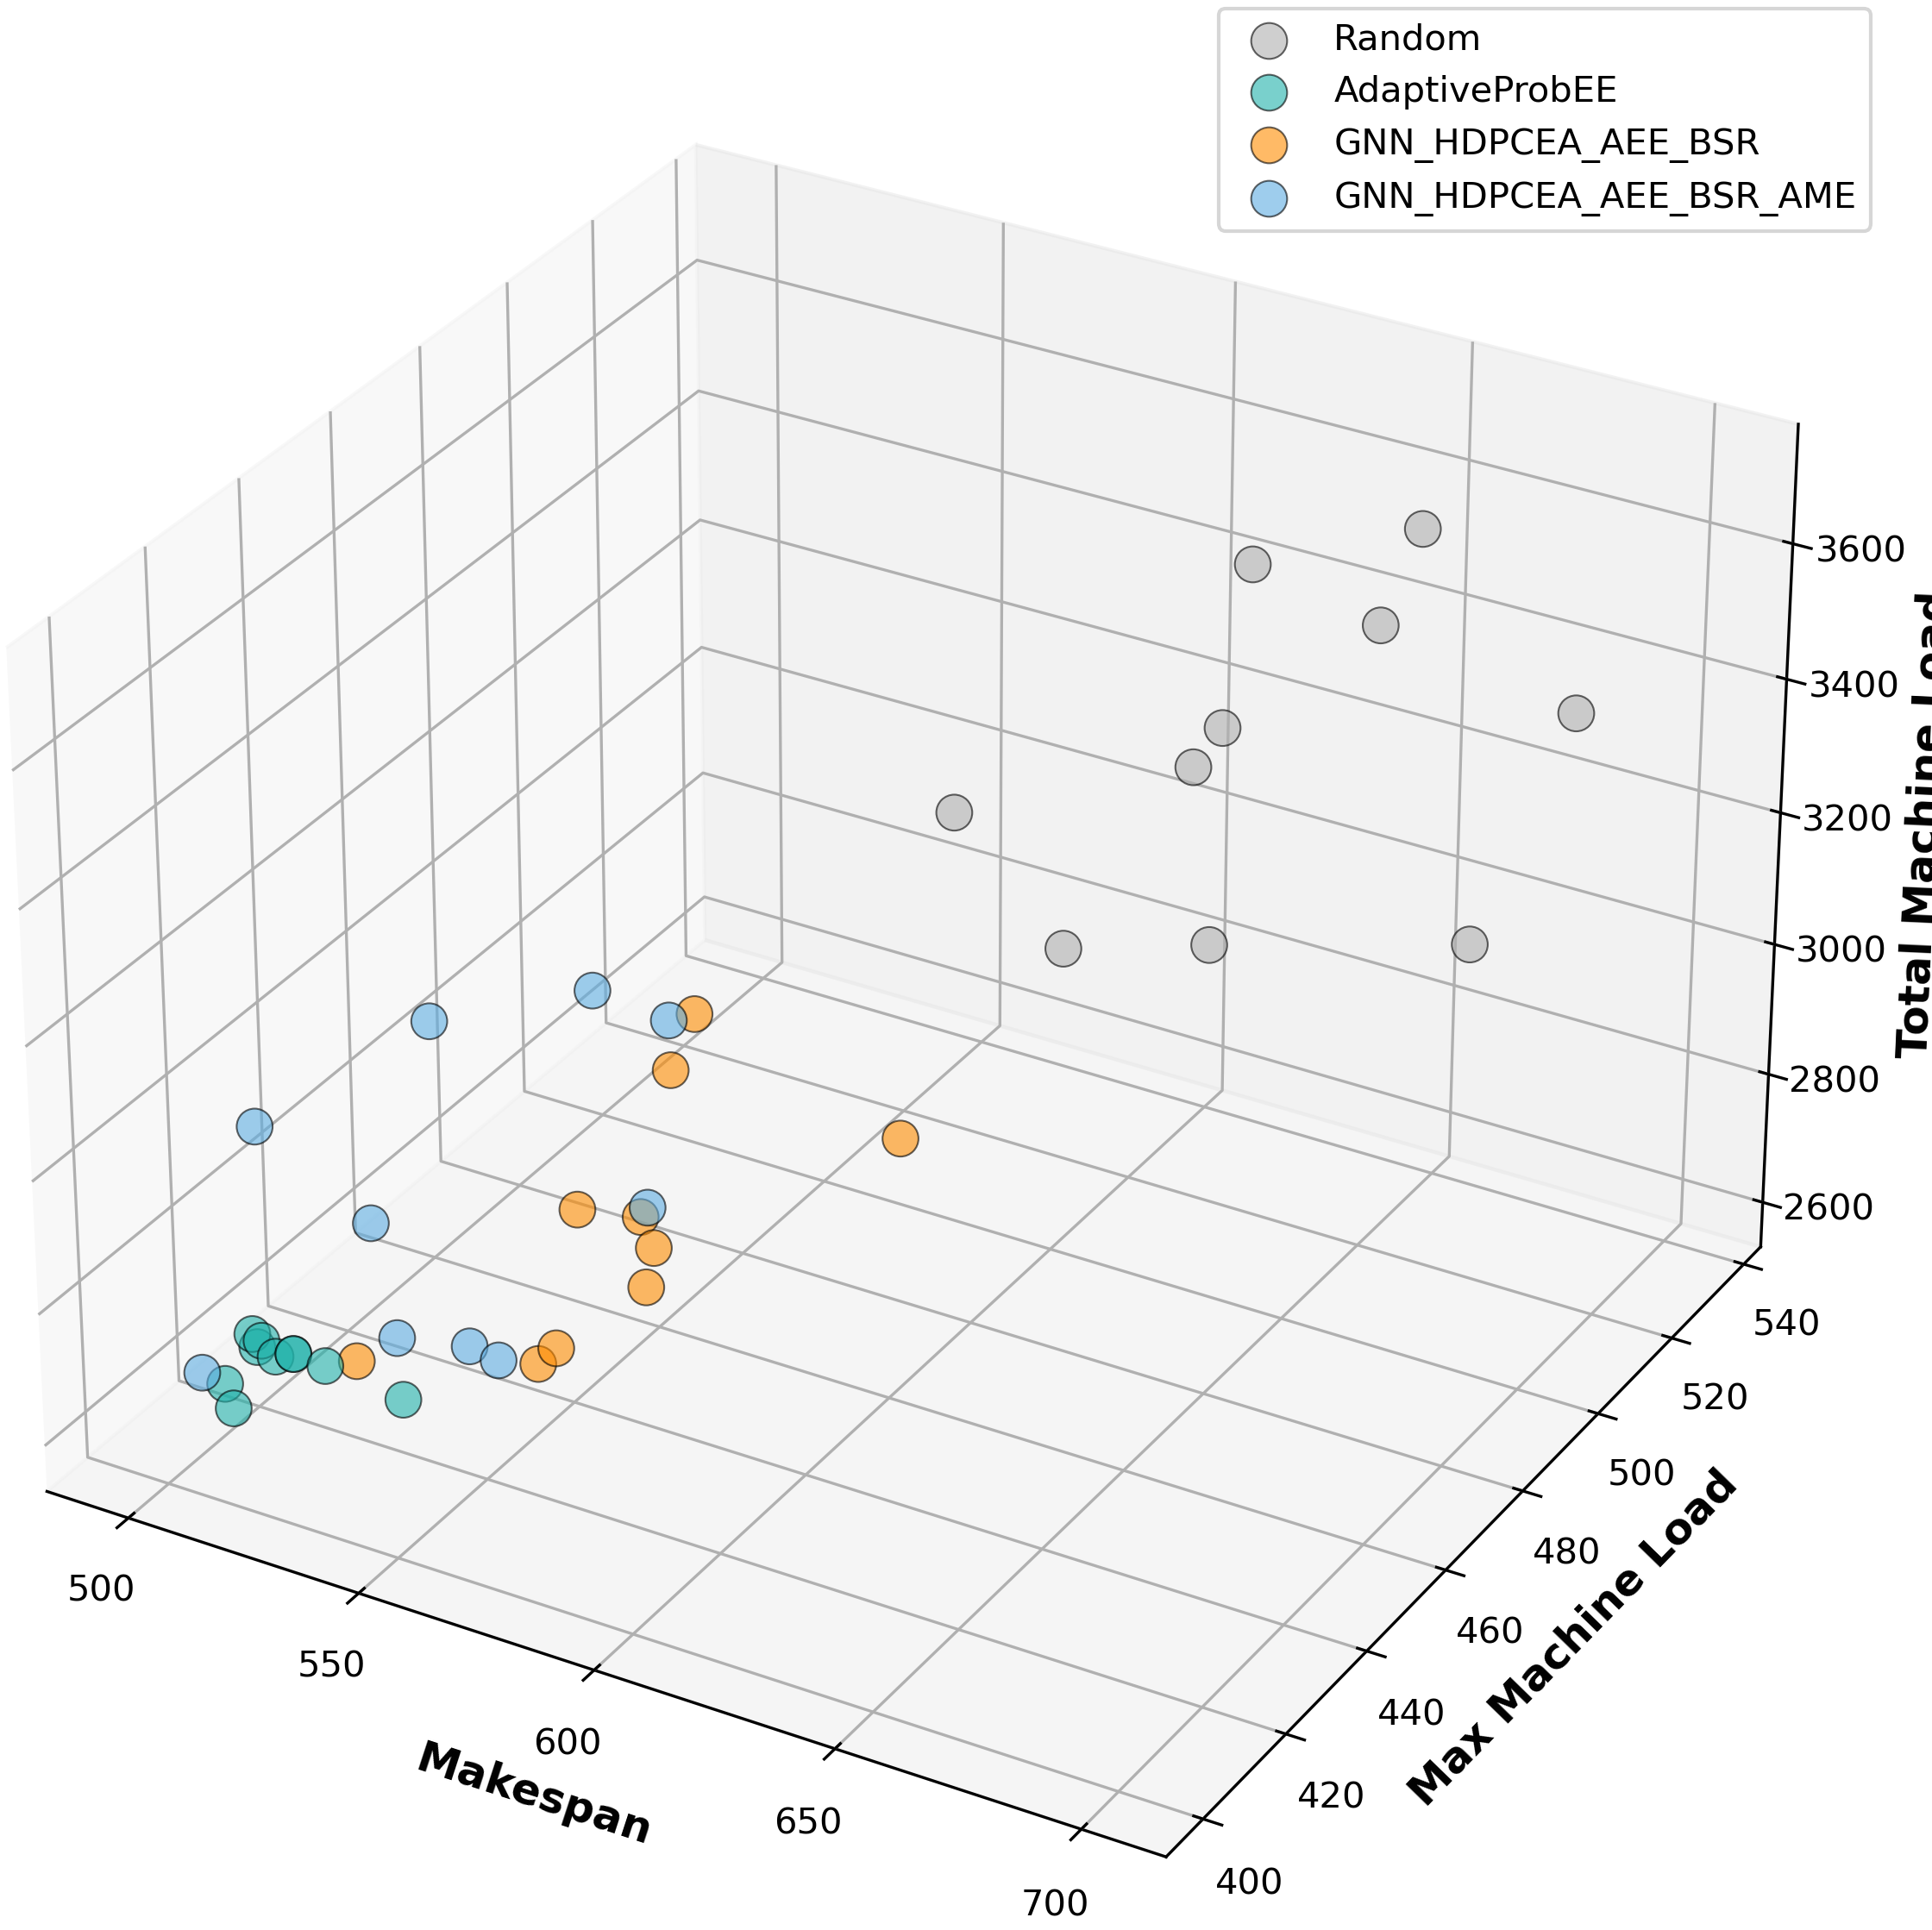
\includegraphics[width=0.49\textwidth]{images/RQ1-pareto_front_3d-val.png}
  \hfill
  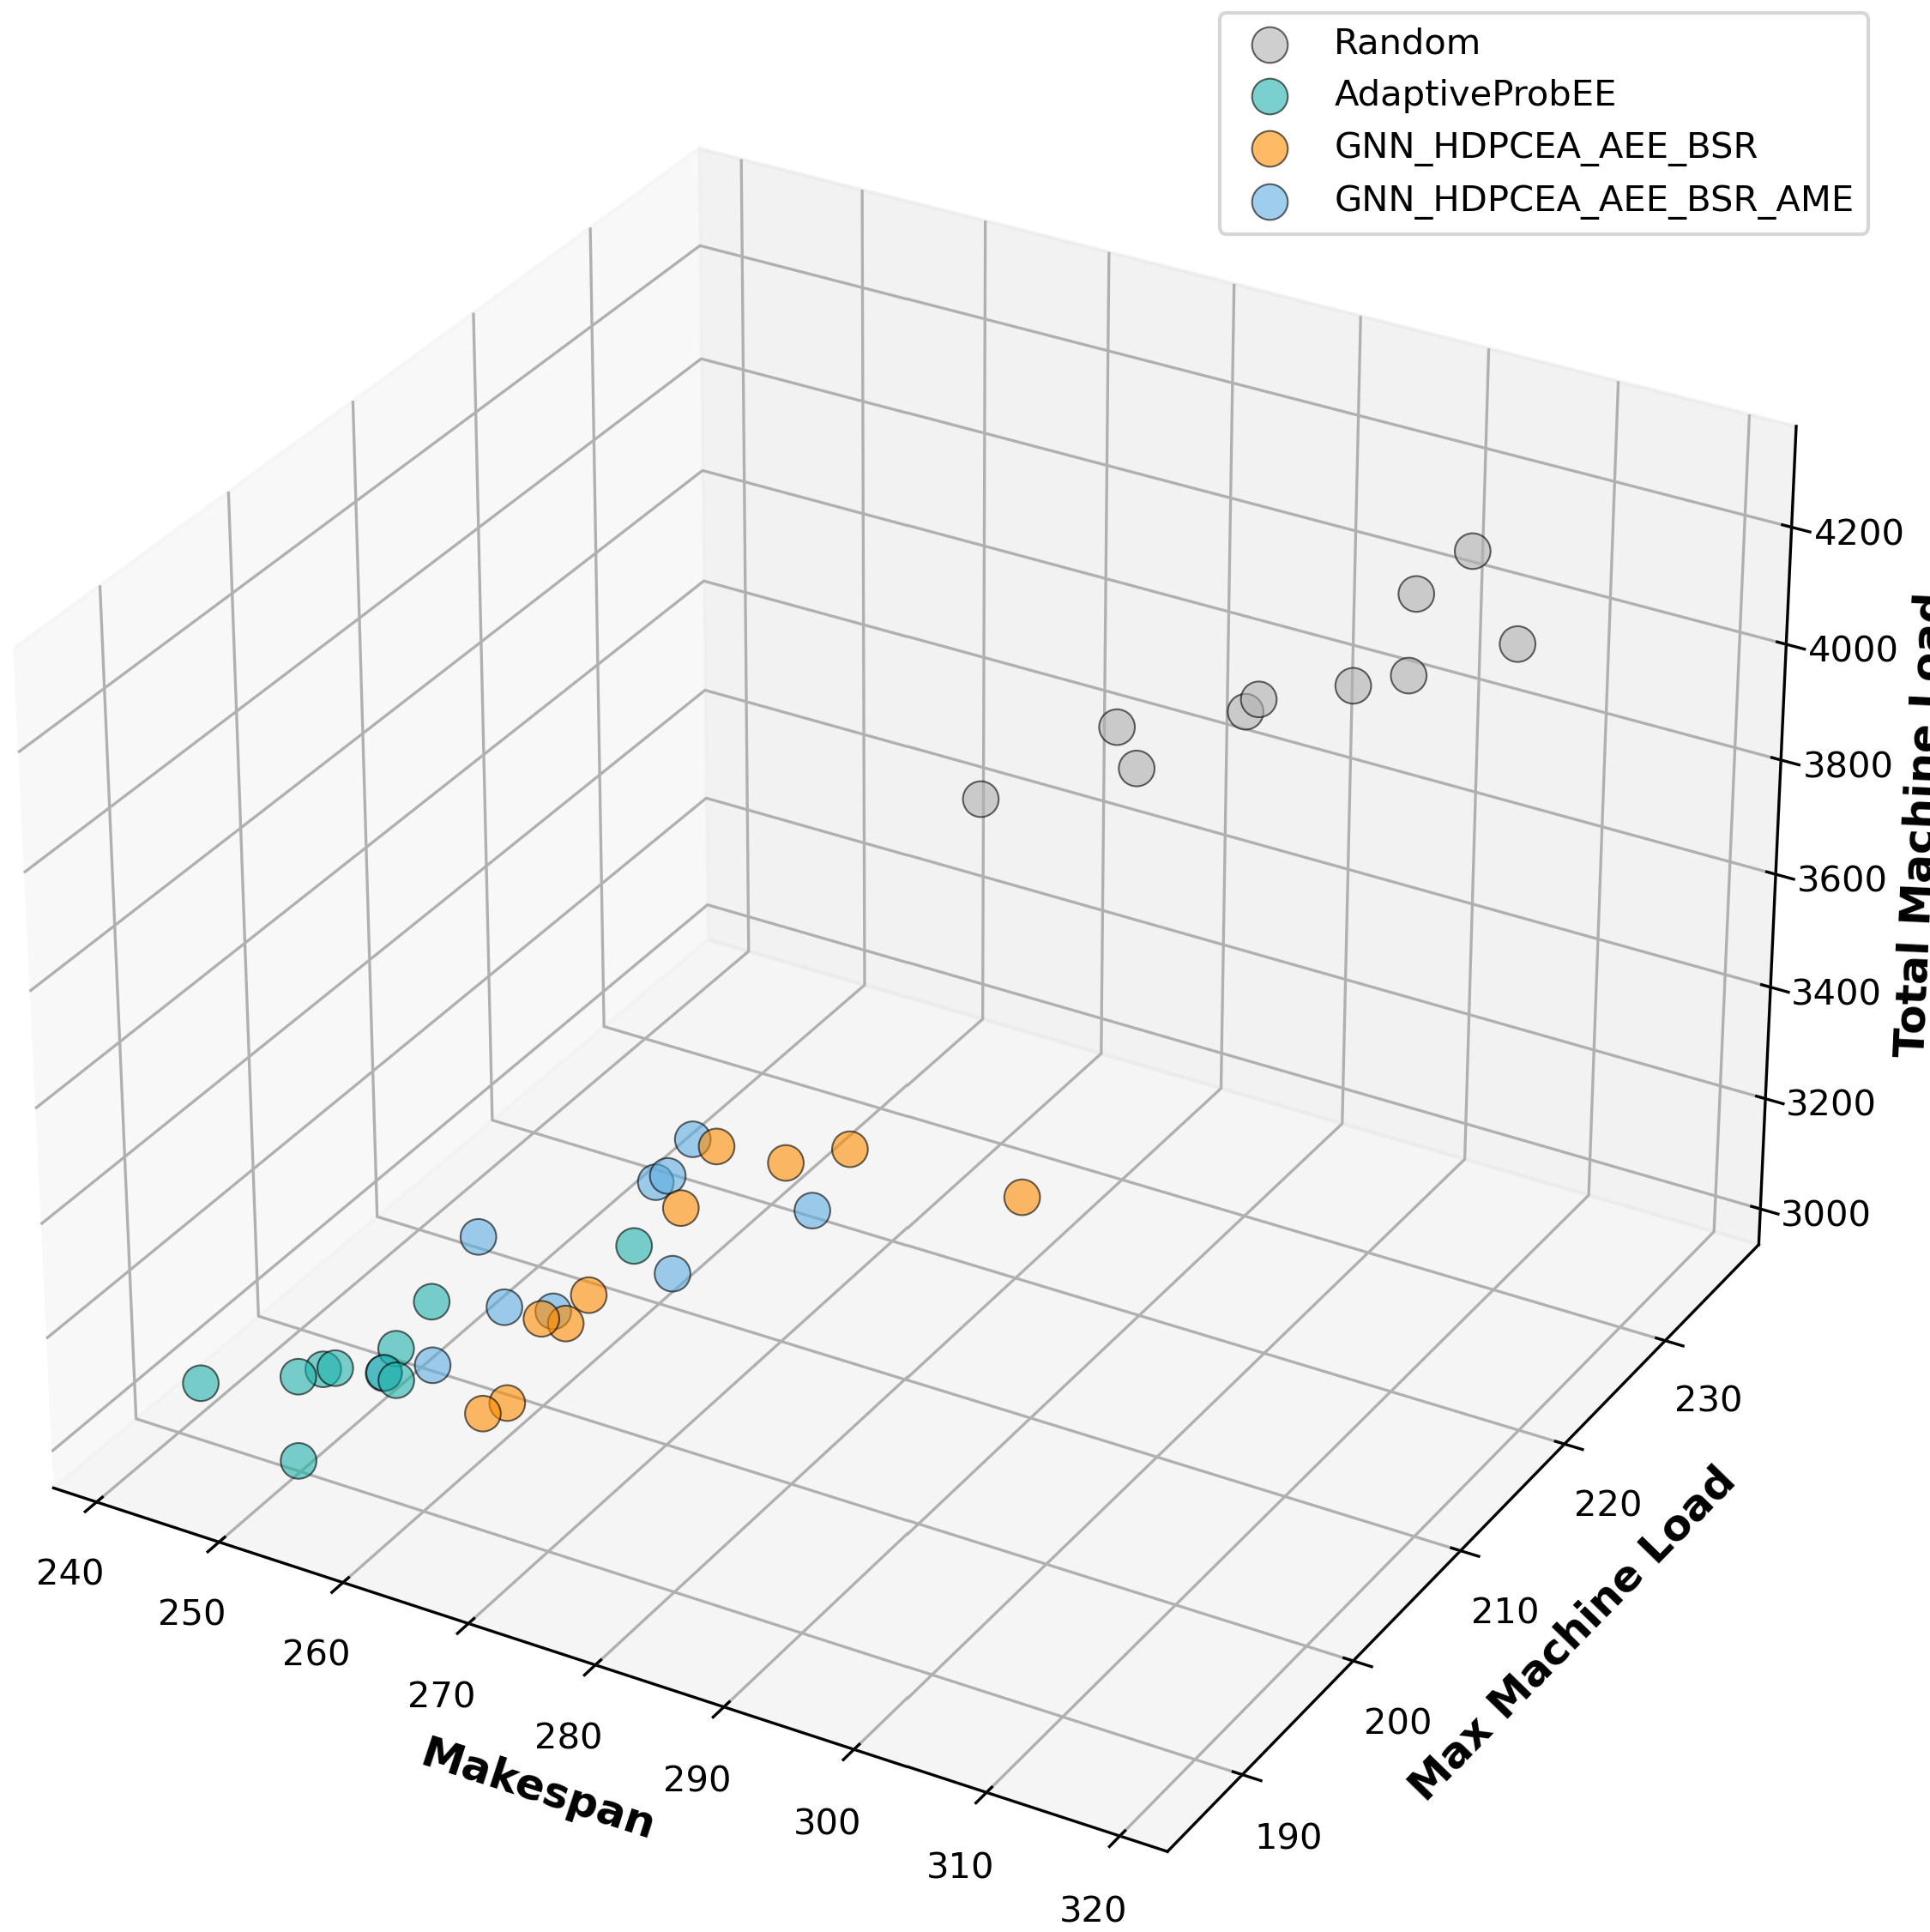
\includegraphics[width=0.49\textwidth]{images/RQ1-pareto_front_3d-test.png}
  \caption{Three-objective Pareto fronts of GNN-HDPCEA-AME on the custom validation set (left) and the BehnkeGeiger benchmark (right).}
  \label{fig:rq1_pareto_3d}
\end{figure*}

%%%%%%%%%%%%%================ RQ1 ====================%%%%%%%%%%%%%%%%

\subsection{Overall framework performance}\label{subsec:rq1}
% 在自定义验证集与 BehnkeGeiger 基准上，将完整的 GNN-HDPCEA-AME 与单种群 NSGA-II（随机初始化与 AdaptiveProbEE 初始化）以及不含 AME 的双种群基线（GNN-HDPCEA-AEE-BSR）进行对比。
% 所有方法的最大迭代代数统一固定为 G=100；双种群方法取 N_MP=N_EP=200，单种群基线采用 200 个个体的种群规模，从而保证每个种群获得相同的单种群预算。
% 如表~\ref{tab:overall_results} 所示，GNN-HDPCEA-AME 在两个数据集上的 HV、IGD、$\Delta$ 与 $\Delta_v$ 均取得最优。
% 在自定义验证集上，其 HV 相较 GNN-HDPCEA-AEE-BSR、AdaptiveProbEE 与随机 NSGA-II 分别提升 15.3\%、30.8\% 与 192.5\%，$\Delta$ 与 $\Delta_v$ 相较 GNN-HDPCEA-AEE-BSR 分别降低 36.7\% 与 31.3\%。
% 其 IGD（16.82）与 AdaptiveProbEE（16.85）基本持平；后者作为面向单目标的初始化方式，已在多个单目标最优解附近聚集，因此与合并参考前沿的接近程度相当，但其明显更大的 $\Delta$ 与 $\Delta_v$ 表明前沿均匀性与稳定性差得多。
% 上述结果表明，在自定义集上，所学初始化、异构双种群结构与 AME 共同提升了前沿质量、分布性与稳定性。
% 尽管 GNN-HDPCEA-AME 在两个数据集上均为最优，但单种群基线在两数据集上的表现并不一致，这有助于厘清所学先验与双种群结构各自的作用。
On both the custom validation set and the BehnkeGeiger benchmark, the full GNN-HDPCEA-AME is compared with single-population NSGA-II (random and AdaptiveProbEE initialization) and the dual-population baseline without AME (GNN-HDPCEA-AEE-BSR, in which AEE denotes the AdaptiveProbEE-initialized MP and BSR the BestSingleRule-initialized EP).
The maximum generation is fixed to $G=100$ for all methods; the dual-population methods use $N_{MP}=N_{EP}=200$, while the single-population baselines use a population of $200$ individuals, so that every population is allocated the same per-population budget.
As shown in Table~\ref{tab:overall_results}, GNN-HDPCEA-AME attains the best HV, IGD, $\Delta$, and $\Delta_v$ among the compared methods on both datasets, whose three-objective Pareto fronts are visualized in Fig.~\ref{fig:rq1_pareto_3d}.
On the custom validation set, its HV improves over GNN-HDPCEA-AEE-BSR, AdaptiveProbEE, and random NSGA-II by 15.3\%, 30.8\%, and 192.5\%, respectively, while $\Delta$ and $\Delta_v$ are reduced by 36.7\% and 31.3\% relative to GNN-HDPCEA-AEE-BSR.
Its IGD ($16.82$) is essentially tied with AdaptiveProbEE ($16.85$); the latter, as a single-objective-oriented initialization, already concentrates near several single-objective optima, so its proximity to the merged reference front is comparable, whereas its much larger $\Delta$ and $\Delta_v$ reveal a far less uniform and less stable front.
These results indicate that, on the custom set, the learned initialization, the heterogeneous dual-population structure, and AME jointly improve front quality, distribution, and stability.
While GNN-HDPCEA-AME is uniformly best on both datasets, the single-population baselines behave differently across them, which helps separate the distinct roles of the learned prior and the dual-population structure.

% 对公开基准的进一步分析可澄清一处表面矛盾。在 BehnkeGeiger 上，AdaptiveProbEE 初始化的单种群 NSGA-II 的 HV 低于随机 NSGA-II（1.62 对 2.02×10^6），但其 IGD 远小于后者（13.70 对 846.66）。
% 这两个指标刻画的侧面不同：HV 奖励被支配区域的延展范围，因此散乱但收敛差的随机前沿反而能在坐标轴方向支配更大的体积；而先验将单种群聚集到高质量折衷区，以牺牲部分延展为代价提升了接近度（IGD）。
% 又因 BehnkeGeiger 实例与合成训练分布存在差异，单独使用的先验在该基准上拓展覆盖的能力被削弱。
% 一旦将先验嵌入异构双种群框架，这一局限即被消除：广度型 MP 与深度型 EP 在双向交换与 AME 的协同下共同恢复并进一步超越覆盖，使 GNN-HDPCEA-AME 在该基准上同时取得最优 HV（3.61×10^6）与最优 IGD（0.7372）。
% 因此，所学先验的作用是提供富含信息的初始化，其全部价值经由双种群协同得以释放，而非充当独立的 HV 提升器。

A closer look at the public benchmark clarifies an apparent anomaly. On BehnkeGeiger, AdaptiveProbEE-seeded single-population NSGA-II reaches a lower HV than random NSGA-II ($1.62$ vs $2.02\times10^{6}$) but a far smaller IGD ($13.70$ vs $846.66$).
The two metrics capture different aspects: HV rewards the extent of the dominated region, so a widely scattered yet poorly converged random front can dominate a larger axis-aligned volume, whereas the prior concentrates the single population around high-quality compromise regions and thus improves proximity (IGD) at the cost of raw spread.
Because the BehnkeGeiger instances also deviate from the synthetic training distribution, the standalone prior is less able to broaden coverage on this benchmark.
This limitation is removed once the prior is embedded in the heterogeneous dual-population framework: the breadth-oriented MP and the depth-oriented EP, coordinated by bidirectional exchange and AME, jointly restore and then surpass coverage, so that GNN-HDPCEA-AME attains both the best HV ($3.61\times10^{6}$) and the best IGD ($0.7372$) among the compared methods on this benchmark.
The learned prior therefore serves as an informative initialization whose full benefit is realized through dual-population cooperation, rather than as a standalone HV booster.
%%%%%%%%%%%%%================ RQ2 ====================%%%%%%%%%%%%%%%%


\subsection{Effectiveness of graph-based prior learning}\label{subsec:rq2}

% GNN 预测器在多目标性能标签数据集上训练。按性能最优规则类别分层采样，以 $r_{train}=0.8$ 划分训练/验证集并保持各类别比例一致；每步处理单个图实例，用梯度累积模拟等效批次，每轮结束后在验证集上全量评估，由学习率调度器决定是否衰减，并保存验证损失最优的检查点；随机种子固定为 42。
% 主要超参数见表~\ref{tab:params}。
% 所有图级读出与卷积深度变体共享相同输入、软标签与训练流程，使表~\ref{tab:gnn_results} 的差异仅来自架构本身。
The GNN predictor is trained on the multi-objective performance-label dataset. The samples are stratified by their best-performing rule class and split into training and validation sets at a ratio of $r_{train}=0.8$, keeping the per-class proportions consistent across both subsets. Each step processes a single graph instance, and an equivalent batch is emulated by gradient accumulation; after every epoch the model is evaluated over the whole validation set, the learning-rate scheduler decides whether to decay the rate, and the checkpoint with the lowest validation loss is retained. The random seed is fixed to 42.
The main GNN hyperparameters are also listed in Table~\ref{tab:params}.
All compared graph-readout and convolution-depth variants share the same input, soft labels, and training protocol, so that the differences in Table~\ref{tab:gnn_results} reflect the architecture alone.

% 表~\ref{tab:gnn_results} 同时报告了训练全程最优值（Best）与第 51--100 轮的收敛后期均值（Mean）。
% NNConv-Attention 在三项分布拟合指标（JS 散度、余弦相似度、Brier 分数）的 Best 与 Mean 上均取得最优，并在 Top-3 准确率上同样领先（Mean 最优，Best 并列最优）。
% 在 Top-3 匹配率上，NNConv-SAG 在两项统计上均略高（约 0.01）；其硬节点选择机制恰好偏向少数排名靠前的规则，但这一微弱优势并未延伸到其他指标。
% 由于在五个规则类别下 Top-3 匹配率与 Top-3 准确率已接近天花板，各模型在这两项指标上差异很小（尤其是 Best），因此收敛后期的 Mean 更能反映模型的稳态表现。
% NNConv-Deep-Attention 在两项统计上均为最差（其 JS 散度 Mean 升至 0.1541、余弦相似度 Mean 降至 0.8331），表明在当前数据规模下单纯增加卷积深度易引发过拟合，从而印证了两层架构的合理性。
% 由于下游进化搜索受益于对竞争性规则的良好校准分布、而非仅仅识别单一最优规则，因此保留全部节点贡献的注意力读出机制更为可取。
Table~\ref{tab:gnn_results} reports both the best value over training (Best) and the converged-stage mean over epochs 51--100 (Mean). NNConv-Attention attains the best result on the three distribution-fitting metrics (JS, Cosine, and Brier) under both Best and Mean, and also the best Top-3 accuracy (best Mean and tied-best Best).
On Top-3 Match, NNConv-SAG is marginally higher under both statistics (by about 0.01); its hard node selection happens to favor a few top-ranked rules, but this slight edge does not carry over to the other metrics.
Because Top-3 Match and Top-3 accuracy are close to their ceiling under five rule classes, the models differ little on these two metrics—especially on Best—so the converged Mean better reflects their stable behavior.
NNConv-Deep-Attention is consistently the worst on both statistics (its JS Mean rises to 0.1541 and its Cosine Mean drops to 0.8331), confirming that simply increasing depth tends to overfit at the current data scale and supporting the two-layer design.
Because the downstream evolutionary search benefits from a calibrated distribution over competitive rules rather than only the single best rule, the attention readout that preserves all node contributions is preferable.
% \begin{table*}[t]
%   \caption{Multi-objective prediction quality on the validation set (converged-stage mean)}
%   \label{tab:gnn_results}
%   \centering
%   \begin{tabular}{lccccc}
%     \toprule
%     Model     & JS $\downarrow$ & Cosine $\uparrow$ & Brier $\downarrow$ & Top3-Match $\uparrow$ & Top3-Acc $\uparrow$ \\
%     \midrule
%     Att.      & \textbf{0.0751} & \textbf{0.8959}   & \textbf{0.0139}    & 0.8067                & \textbf{0.8633}     \\
%     SAG       & 0.0779          & 0.8924            & 0.0143             & \textbf{0.8132}       & 0.8630              \\
%     Set2Set   & 0.0766          & 0.8906            & 0.0146             & 0.8058                & 0.8626              \\
%     Mean      & 0.0921          & 0.8910            & 0.0147             & 0.7993                & 0.8614              \\
%     Deep-Att. & 0.1541          & 0.8331            & 0.0230             & 0.7158                & 0.8612              \\
%     \bottomrule
%   \end{tabular}

%   \vspace{2pt}
%   {\footnotesize\raggedright Note: Att.\ and Deep-Att.\ are short for NNConv-Attention and NNConv-Deep-Attention; Set2Set, SAG, and Mean correspond to NNConv-Set2Set, NNConv-SAG, and NNConv-Mean, respectively. In each column, the bold value marks the best result.\par}
% \end{table*}
\begin{table*}[t]
  \caption{Multi-objective prediction quality on the validation set.}
  \label{tab:gnn_results}
  \centering
  \footnotesize
  \setlength{\tabcolsep}{4pt}
  \begin{tabular*}{\textwidth}{@{\extracolsep{\fill}} l cc cc cc cc cc}
    \toprule
    \multirow{2}{*}{Model}
    & \multicolumn{2}{c}{JS $\downarrow$}
    & \multicolumn{2}{c}{Cosine $\uparrow$}
    & \multicolumn{2}{c}{Brier $\downarrow$}
    & \multicolumn{2}{c}{Top3-Match $\uparrow$}
    & \multicolumn{2}{c}{Top3-Acc $\uparrow$} \\
    \cmidrule(lr){2-3}\cmidrule(lr){4-5}\cmidrule(lr){6-7}\cmidrule(lr){8-9}\cmidrule(lr){10-11}
    & Best & Mean & Best & Mean & Best & Mean & Best & Mean & Best & Mean \\
    \midrule
    Att.      & \textbf{0.0723} & \textbf{0.0751} & \textbf{0.8981} & \textbf{0.8959} & \textbf{0.0136} & \textbf{0.0139} & 0.8150          & 0.8067          & \textbf{0.8736} & \textbf{0.8633} \\
    SAG       & 0.0743          & 0.0779          & 0.8959          & 0.8924          & 0.0139          & 0.0143          & \textbf{0.8260} & \textbf{0.8132} & \textbf{0.8736} & 0.8630          \\
    Set2Set   & 0.0732          & 0.0766          & 0.8934          & 0.8906          & 0.0143          & 0.0146          & 0.8186          & 0.8058          & 0.8681          & 0.8626          \\
    Mean      & 0.0779          & 0.0921          & 0.8915          & 0.8910          & 0.0143          & 0.0147          & 0.8040          & 0.7993          & 0.8681          & 0.8614          \\
    Deep-Att. & 0.1116          & 0.1541          & 0.8772          & 0.8331          & 0.0165          & 0.0230          & 0.7948          & 0.7158          & 0.8735          & 0.8612          \\
    \bottomrule
  \end{tabular*}

  \vspace{2pt}
  \footnotesize\raggedright
  Note: Att./Deep-Att./Set2Set/SAG/Mean denote NNConv with attention, deep (3-layer) attention, Set2Set, SAG, and mean pooling, respectively.
  For each metric, ``Best'' is the best value over all epochs and ``Mean'' the average over epochs 51--100.
  Top3-Match and Top3-Acc are near their ceiling under five rule classes, so the epoch-averaged Mean is more discriminative than Best.
\end{table*}

% GNN 的作用是减少盲目初始化，而非直接输出最终调度。
From a manufacturing decision-support perspective, the GNN does not output a final schedule; it reduces blind initialization by identifying rule combinations that suit the structure of a new FJSP instance, letting the evolutionary solver start from a more informed region while retaining the ability to explore trade-off schedules.


%%%%%%%%%%%%%================ RQ3 ====================%%%%%%%%%%%%%%%%


\subsection{Rationality of heterogeneous population roles}\label{subsec:rq3}
% 沿用 RQ1 的四项前沿指标，并辅以三目标的均值统计以考察 MP/EP 的角色分工。
This experiment uses the same four Pareto-front metrics as Section~\ref{subsec:rq1} (HV, IGD, $\Delta$, $\Delta_v$). In addition, for the single-population initialization strategies the per-objective averages of makespan, maximum machine workload, and total workload (Table~\ref{tab:single_pop}) are reported to identify which initialization suits the breadth-oriented MP and which the core-focused EP; the dual-population combinations are then compared on the four front metrics (Table~\ref{tab:dual_pop}).

% 先在单种群下观察各初始化策略，定位 MP 与 EP 的候选角色。
Table~\ref{tab:single_pop} first reports single-population NSGA-II under different initialization strategies. BestSingleRule, although not the strongest on any single objective, attains the best HV and the best $\Delta_v$, indicating a well-covered and stable compromise front; AdaptiveProbEE attains the best IGD and explores the single-objective directions more broadly. This contrast motivates the heterogeneous pairing: AdaptiveProbEE for the breadth-oriented MP and BestSingleRule for the core-focused EP.

% \begin{table*}[t]
%   \caption{Single-population NSGA-II under different initialization strategies (validation set)}
%   \label{tab:single_pop}
%   \centering
%   \begin{tabular}{lrrrr}
%     \toprule
%     Initialization     & HV $\uparrow$               & $\Delta \downarrow$ & $\Delta_v \downarrow$ & IGD $\downarrow$ \\
%     \midrule
%     Random             & $1.93{\times}10^7$          & 12.7339             & 5.8543                & 703.71             \\
%     AdaptiveWeighted   & $4.28{\times}10^7$          & 13.4858             & 5.5609                & 34.21              \\
%     UniformMixed       & $4.00{\times}10^7$          & 13.3504             & 5.4539                & 31.22              \\
%     BestSingleRule     & $\mathbf{4.62{\times}10^7}$ & 13.1510             & \textbf{4.7173}       & 44.43              \\
%     SoftmaxTemperature & $2.73{\times}10^7$          & \textbf{12.5120}    & 5.3677                & 33.74              \\
%     AdaptiveProbEE     & $3.61{\times}10^7$          & 12.9599             & 5.0782                & \textbf{24.12}     \\
%     \bottomrule
%   \end{tabular}
% \end{table*}
\begin{table*}[t]
  \caption{Single-population NSGA-II under different initialization strategies (validation set)}
  \label{tab:single_pop}
  \centering
  \footnotesize
  \setlength{\tabcolsep}{4pt}
  \begin{tabular*}{\textwidth}{@{\extracolsep{\fill}} l rrrr rrr}
    \toprule
    Initialization   & HV $\uparrow$               & $\Delta \downarrow$ & $\Delta_v \downarrow$ & IGD $\downarrow$ & Mksp$^\ast$ $\downarrow$ & MaxLoad$^\ast$ $\downarrow$ & TotalLoad$^\ast$ $\downarrow$ \\
    \midrule
    Random           & $1.93{\times}10^7$          & 12.7339             & 5.8543                & 703.71             & 770.35          & 624.10          & 3484.15          \\
    AdaptiveWeighted & $4.28{\times}10^7$          & 13.4858             & 5.5609                & 34.21              & 697.60          & 576.05          & 2923.25          \\
    UniformMixed     & $4.00{\times}10^7$          & 13.3504             & 5.4539                & 31.22              & 699.65          & 578.05          & 2923.10          \\
    BestSingleRule   & $\mathbf{4.62{\times}10^7}$ & 13.1510             & \textbf{4.7173}       & 44.43              & 713.10          & 576.00          & 2935.70          \\
    AdaptiveProbEE   & $3.61{\times}10^7$          & \textbf{12.9599}    & 5.0782                & \textbf{24.12}     & \textbf{687.60} & \textbf{563.75} & \textbf{2920.80} \\
    \bottomrule
  \end{tabular*}

  \vspace{2pt}
  \footnotesize\raggedright
  $^\ast$ Mksp, MaxLoad, and TotalLoad denote the average of the best (minimum) makespan, maximum machine load, and total load over independent runs, respectively (lower is better).
\end{table*}

% 再在双种群下比较不同 MP/EP 组合（同规模），说明性能差异源于功能搭配而非规模。
Table~\ref{tab:dual_pop} then compares dual-population variants under an equal per-population budget ($N_{MP}=N_{EP}=200$, $G=100$), where SFM denotes a temperature-smoothed prior-weighted initialization (SoftmaxTemperature) and the suffix order denotes the MP/EP assignment. Across the four combinations, HV varies from $1.15\times10^8$ to $1.39\times10^8$ and IGD spans roughly fivefold (44.6 to 224.2), showing that the performance gap stems from the MP/EP functional pairing rather than the total population size. Note that the single-population rows (AdaptiveProbEE, Random) carry larger HV here than the same methods in Table~\ref{tab:single_pop}: because Table~\ref{tab:dual_pop} also contains the more extended dual-population fronts, the shared reference point $\mathbf{r}=1.1\cdot(\max f_1,\max f_2,\max f_3)$ is pushed outward and inflates every HV in this table. The two single-population rows therefore serve only as positioning references within Table~\ref{tab:dual_pop} and are not directly comparable to Table~\ref{tab:single_pop}. The adopted GNN-HDPCEA-AEE-BSR combines a large HV ($1.36\times10^8$) with a low IGD (46.99), whereas GNN-HDPCEA-SFM-AEE attains a slightly higher HV but an IGD above 224, indicating a broader yet less accurate front. The bidirectional exchange lets the two populations share complementary information, and the role separation turns the convergence-diversity tension into explicit cooperation, yielding a more stable set of Pareto schedules covering different priorities such as urgent delivery, bottleneck relief, or workload balance.

\begin{table*}[t]
  \caption{Single- vs. dual-population NSGA-II with different MP/EP combinations (validation set)}
  \label{tab:dual_pop}
  \centering
  \begin{tabular}{lrrrr}
    \toprule
    Strategy                & HV $\uparrow$               & $\Delta \downarrow$ & $\Delta_v \downarrow$ & IGD $\downarrow$ \\
    \midrule
    AdaptiveProbEE (single) & $9.79{\times}10^7$          & 24.3051             & 9.5747                & 85.31            \\
    Random (single)         & $4.25{\times}10^7$          & \textbf{21.2775}    & \textbf{7.1460}       & 1565.19          \\
    GNN-HDPCEA-BSR-AEE      & $1.15{\times}10^8$          & 27.4785             & 18.4111               & \textbf{44.56}   \\
    GNN-HDPCEA-SFM-AEE      & $\mathbf{1.39{\times}10^8}$ & 22.4481             & 11.2872               & 224.21           \\
    GNN-HDPCEA-AEE-BSR      & $1.36{\times}10^8$          & 26.1621             & 15.5279               & 46.99            \\
    GNN-HDPCEA-AEE-SFM      & $1.16{\times}10^8$          & 27.5454             & 12.7385               & 223.45           \\
    \bottomrule
  \end{tabular}
\end{table*}





\subsection{Manufacturing implications and limitations}\label{subsec:discussion}
% 本研究亦存在若干局限。其一，实验基于合成与公开基准实例，而非真实生产线。
% 其二，$W_{\mathrm{total}}$ 是一种负荷相关代理，并未涵盖能耗的全部组成，如机器空载能耗、换刀或分时电价。
% 其三，当前框架聚焦于静态 FJSP，尚未纳入动态到达、机器故障与紧急订单插入。
% 这些局限指向面向动态制造环境与更精细能耗感知调度模型的自然扩展方向。
The proposed framework can be used as an offline-trained and online-applied scheduling decision-support module. Historical or simulated scheduling instances are used to train the GNN predictor offline. For a new production order set, the trained predictor rapidly provides instance-aware dispatching-rule priors, and the dual-population evolutionary solver returns a set of trade-off schedules. Production planners can then choose schedules according to delivery urgency, bottleneck machine availability, or workload-balance requirements.

The current study also has limitations.
First, the experiments are based on synthetic and public benchmark instances rather than a live production line.
Second, $W_{\mathrm{total}}$ is a workload-related proxy and does not capture all components of energy consumption, such as machine idle energy, tool change, or time-of-use electricity tariffs.
Third, the current framework focuses on static FJSP; dynamic arrivals, machine breakdowns, and urgent order insertion are not yet included.
Fourth, the experiments compare the framework against single-population NSGA-II and reduced dual-population variants (homogeneous initialization and without AME) so as to isolate the contribution of each proposed component; a broader benchmarking against classical multi-objective algorithms such as NSGA-III and MOEA/D is left to future work.
These limitations suggest natural future extensions toward dynamic manufacturing environments, more detailed energy-aware scheduling models, and comprehensive comparison with classical multi-objective optimizers.









\section{Conclusions}\label{sec:conclusion}

This paper developed a heterogeneous dual-population evolutionary optimization approach for multi-objective FJSP, in which an instance-specific learned prior strengthens evolutionary search on two fronts. A static heterogeneous disjunctive graph and an edge-conditioned GNN predictor learn instance-aware dispatching-rule distributions from offline scheduling data, and the learned distribution guides the initialization of two complementary populations: a main population for Pareto-front breadth and an exploratory population for intensified search around a high-quality core. Bidirectional exchange and AME coordinate the two populations during optimization.

% 在合成实例与公开的 BehnkeGeiger 基准上，所提方法在帕累托前沿质量与分布稳定性上均优于单种群与双种群基线。在自定义验证集上，完整框架的 HV 相较无 AME 的双种群基线、单种群学习先验与随机 NSGA-II 分别提升 15.3\%、30.8\% 与 192.5\%，间距 $\Delta$ 与其方差 $\Delta_v$ 分别降低 36.7\% 与 31.3\%。结果表明，以实例特定学习先验与异构双种群结构增强多目标进化搜索可带来一致且互补的增益。
Experiments on synthetic instances and the public BehnkeGeiger benchmark showed that the approach improved Pareto-front quality and distribution stability compared with single-population and dual-population baselines. On the custom validation set, the full framework improved HV by 15.3\% over the dual-population baseline without AME, by 30.8\% over the single-population learned prior, and by 192.5\% over random NSGA-II, while reducing the spacing $\Delta$ and its variance $\Delta_v$ by 36.7\% and 31.3\%. These results show that strengthening multi-objective evolutionary search with an instance-specific learned prior and a heterogeneous dual-population structure yields consistent and complementary gains.

Future work will extend the framework to dynamic FJSP with machine breakdowns, order arrivals, and changing processing conditions. More realistic energy-consumption objectives can also be incorporated beyond workload-based proxies. Another promising direction is to combine learned scheduling priors with explainable decision-support interfaces so that production planners can understand why different Pareto schedules are recommended.

\section*{Statements and Declarations}

\subsection*{Funding}

The authors declare that no funds, grants, or other support were received during the preparation of this manuscript.

\subsection*{Competing interests}

The authors have no relevant financial or non-financial interests to disclose.

\subsection*{Author contributions}

Changqi Han contributed to conceptualization, methodology, software, validation, investigation, and writing of the original draft. Jie He contributed to supervision, methodology, and manuscript review and editing. Shihong Duan contributed to supervision and manuscript review and editing. All authors read and approved the final manuscript.

\subsection*{Data availability}

The datasets generated and analyzed during the current study are available from the corresponding author on reasonable request.

\subsection*{Code availability}

The code generated during the current study is not publicly available, as it forms part of ongoing research and further development. The methodology is described in detail in this paper; further clarification is available from the corresponding author on reasonable request.

\bibliography{references}

\end{document}
